
\begin{table}
\centering
\begin{tabular}{l l l}
\hline
\textbf{TCR / Ab} & \textbf{(PDBid, WT peptide)} & \textbf{MHC allele} \\
\hline \hline
1G4 TCR & (2BNR~\cite{chen_structural_2005}, SLLMWITQC); (2BNQ~\cite{chen_structural_2005},
SLLMWITQV) & HLA-A*02:01 \\
A6 TCR & (1AO7~\cite{Garboczi1996-fr}, LLFGYPVYV); (1QSF~\cite{ding_four_1999}, LLFGYPVAV) &
HLA-A*02:01 \\
\hline
TCR1 &                    (5D2N~\cite{Yang2015-cj}, NLVPMVATV) & HLA-A*02:01 \\
TCR2 &               (AF3 model, NLVPMVATV) & HLA-A*02:01 \\
TCR3 &               (AF3 model, NLVPMVATV) & HLA-A*02:01 \\
TCR4 &               (AF3 model, IMDQVPFSV) & HLA-A*02:01 \\
TCR5 &               (AF3 model, IMDQVPFSV) & HLA-A*02:01 \\
TCR6 &               (AF3 model, IMDQVPFSV) & HLA-A*02:01 \\
TCR7 &               (AF3 model, GRLKALCQR) & HLA-B*27:05 \\
H2-scDb (Fab) &                    (6W51~\cite{Hsiue2021-ag}, HMTEVVRHC) & HLA-A*02:01 \\
\hline
\end{tabular}
\figcaption{Structure templates used for the binding affinity and T-cell activity analyses.}{
\normalfont{The first two rows contain information related to the analyses on binding affinity data,
the rest are related to T-cell activity data. Every structure identified by a 4-letter PDBid was
downloaded from the Protein Data Bank. The raw PDB file for 5D2N~\cite{Yang2015-cj} has two copies
of the TCR-pMHC complex, so we deleted one before running any analysis. Similarly, the raw PDB file
for 6W51~\cite{Hsiue2021-ag} has the Antibody and pMHC coordinates of two different copies within
the crystal, so we expanded the crystal using PyMOL's \texttt{symexp} command and kept a single
bound Antibody-pMHC complex. The sequence inputs used to fold TCR-pMHC complexes with
AlphaFold3~\cite{Abramson2024-jp} can be found in Dataset~\ref{dataset:af3_sequences}}.\\\\\\
}
\label{table:affinity_and_activity_info}
\end{table}



\begin{table}[ht]
\centering
\begin{tabular}{l l c c}
\hline
Model type & Model & 1G4 TCR & A6 TCR \\
\hline \hline
\multirow{3}{*}{Substitution Matrix} & BLOSUM62 & {\bf\underline{0.83}} \scriptsize{(0.00)} & 0.56*
\scriptsize{(0.02)} \\
& Luksza et al. $M$ & 0.44* \scriptsize{(0.12)} & 0.24 \scriptsize{(0.38)} \\
& Luksza et al. $d \cdot M$ & 0.48* \scriptsize{(0.08)} & 0.29 \scriptsize{(0.27)} \\
\hline
\multirow{2}{*}{Structure Predictor} & TCRdock & 0.62* \scriptsize{(0.02)} & {\bf\underline{0.88}}
\scriptsize{(0.00)} \\
 & TCRdock-{\em no template} & 0.25 \scriptsize{(0.39)} & -0.14 \scriptsize{(0.62)} \\
\hline
 \multirow{2}{*}{Sequence-based} &TAPIR &  0.29 \scriptsize{(0.32)} & 0.35 \scriptsize{(0.19)} \\
 & NetTCR-2.2 & -0.25 \scriptsize{(0.40)} & -0.27 \scriptsize{(0.36)} \\
\hline
\multirow{9}{*}{Structure-based} & ESM-IF1 & 0.38* \scriptsize{(0.17)} & 0.17 \scriptsize{(0.53)} \\
& ProteinMPNN 0.02 Pep 1-by-1 & -0.01 \scriptsize{(0.97)} & 0.49 \scriptsize{(0.05)} \\
 & ProteinMPNN 0.20 Pep 1-by-1 & 0.12 \scriptsize{(0.69)} & 0.29 \scriptsize{(0.27)} \\
& ProteinMPNN 0.02 Pep  & -0.01 \scriptsize{(0.97)} & 0.49 \scriptsize{(0.06)} \\
 & ProteinMPNN 0.20 Pep & 0.14 \scriptsize{(0.63)} & 0.29 \scriptsize{(0.27)} \\
 & ProteinMPNN 0.02 Pep and TCR & 0.07 \scriptsize{(0.81)} & 0.54 \scriptsize{(0.03)} \\
 & ProteinMPNN 0.20 Pep and TCR & -0.08 \scriptsize{(0.79)} & 0.26 \scriptsize{(0.33)} \\
\hline
 \multirow{6}{*}{Structure-based} & HERMES-{\em fixed} 0.00 & 0.29 \scriptsize{(0.31)} & 0.63*
 \scriptsize{(0.01)} \\
 & HERMES-{\em fixed} 0.50 & 0.19 \scriptsize{(0.51)} & -0.28 \scriptsize{(0.29)} \\
 & HERMES-{\em relaxed} 0.00 & 0.72* \scriptsize{(0.00)} & 0.56* \scriptsize{(0.03)} \\
 & HERMES-{\em relaxed} 0.50 & 0.65* \scriptsize{(0.01)} & 0.06 \scriptsize{(0.83)} \\
 & HERMES-{\em relaxed}-min\_energy 0.00 & 0.58* \scriptsize{(0.03)} & 0.71* \scriptsize{(0.00)} \\
 & HERMES-{\em relaxed}-min\_energy 0.50 & 0.52* \scriptsize{(0.06)} & 0.51 \scriptsize{(0.04)} \\
\hline
\end{tabular}
\figcaption{Benchmarking of models for predicting TCR-pMHC binding affinities.}{
\normalfont{The table lists the Spearman correlation~$\rho \,{\rm (p-value)}$ of models' predictions
against experimentally measured binding affinities for (i) 1G4 TCR in complex with HLA-A*02:01
binding to the variants of the NY-ESO-1 peptide, and (ii) the A6 TCR in complex with HLA-A*02:01
binding to the variants of the Tax peptide. The HERMES model names specify the scoring scheme
(fixed, relaxed, and relaxed with peptide energy computed from the relaxed conformation with the
minimum Rosetta energy), and the noise amplitude (in \AA) injected to the coordinates of the
structure data during training. Similarly, the ProteinMPNN model names capture scoring scheme
(1-by-1 (eq.~\ref{eq:peplogp_proteinmpnn}), the whole peptide
(eq.~\ref{eq:peplogp_proteinmpnn_pep}), and the peptide and TCR interface together
(eq.~\ref{eq:peplogp_proteinmpnn_tcr_and_pep})), and the noise amplitude injected to the training
data. We show in \textbf{bold} the best model for each dataset, and any model whose performance is
not significantly different from the best model (p-value$>0.05$ for the difference in the Fisher's
z-transformed Spearman correlations) is indicated with an asterisk (*).
}}
\label{table:spearmanr_affinity}
\end{table}




\begin{table}[ht]
\centering
\resizebox{1.0\textwidth}{!}{
\begin{tabular}{ l l c c c c c c c c c }
\hline
Model type & Model & H2-scDb (Fab) & TCR1 & TCR2 & TCR3 & TCR4 & TCR5 & TCR6 & TCR7 \\
 \hline \hline
\multirow{3}{*}{Sub. Matrix} & BLOSUM62 & -0.05 \scriptsize{(0.52)} & -0.07 \scriptsize{(0.47)} &
0.14 \scriptsize{(0.20)} & 0.38 \scriptsize{(0.00)} & 0.33* \scriptsize{(0.01)} & 0.42*
\scriptsize{(0.00)} & 0.55* \scriptsize{(0.00)} & -0.01 \scriptsize{(0.89)} \\
& Luksza et al. $M$ & 0.19 \scriptsize{(0.02)} & $^\dagger$0.25 \scriptsize{(0.01)} & $^\dagger$0.39
\scriptsize{(0.00)} & $^\dagger$0.53* \scriptsize{(0.00)} & $^\dagger$0.25* \scriptsize{(0.03)} &
$^\dagger$0.27 \scriptsize{(0.00)} & $^\dagger$0.36* \scriptsize{(0.00)} & $^\dagger$0.01
\scriptsize{(0.94)} \\
& Luksza et al. $d \cdot M$ & 0.46* \scriptsize{(0.00)} & $^\dagger$0.50* \scriptsize{(0.00)} &
$^\dagger$0.66* \scriptsize{(0.00)} & $^\dagger$0.40 \scriptsize{(0.00)} & $^\dagger${\bf
\underline{0.38}} \scriptsize{(0.00)} & $^\dagger$ {\bf \underline{0.55}} \scriptsize{(0.00)} &
$^\dagger${0.42}* \scriptsize{(0.00)} & $^\dagger$0.27* \scriptsize{(0.00)} \\
\hline
\multirow{2}{*}{Struc. Pred.} & TCRdock & N/A & 0.02 \scriptsize{(0.83)} & 0.13 \scriptsize{(0.24)}
& 0.21 \scriptsize{(0.03)} & 0.18 \scriptsize{(0.15)} & -0.02 \scriptsize{(0.83)} & 0.19
\scriptsize{(0.04)} & 0.06 \scriptsize{(0.50)} \\
& TCRdock-{\em no template} & N/A & -0.03 \scriptsize{(0.77)} & 0.44 \scriptsize{(0.00)} & 0.11
\scriptsize{(0.27)} & -0.22 \scriptsize{(0.08)} & 0.28 \scriptsize{(0.00)} & 0.14
\scriptsize{(0.14)} & 0.06 \scriptsize{(0.50)} \\
\hline
\multirow{4}{*}{Seq.-based} & TAPIR & N/A & 0.36 \scriptsize{(0.00)} & 0.36 \scriptsize{(0.00)} &
-0.00 \scriptsize{(0.97)} & 0.12 \scriptsize{(0.32)} & 0.39* \scriptsize{(0.00)} & 0.08
\scriptsize{(0.42)} & -0.01 \scriptsize{(0.94)} \\
& NetTCR-2.2 & N/A & -0.05 \scriptsize{(0.59)} & 0.20 \scriptsize{(0.06)} & 0.36 \scriptsize{(0.00)}
& -0.21 \scriptsize{(0.09)} & 0.23 \scriptsize{(0.01)} & 0.20 \scriptsize{(0.03)} & -0.22
\scriptsize{(0.02)} \\
& TULIP & N/A & 0.12 \scriptsize{(0.24)} & 0.18 \scriptsize{(0.09)} & -0.12 \scriptsize{(0.20)} &
0.04 \scriptsize{(0.73)} & 0.24 \scriptsize{(0.00)} & 0.29 \scriptsize{(0.00)} & N/A \\
& TULIP* (from~\cite{Meynard-Piganeau2024-po}) & N/A & 0.47* \scriptsize{(0.00)} & 0.44
\scriptsize{(0.00)} & 0.14 \scriptsize{(0.07)} & 0.23* \scriptsize{(0.00)} & 0.20
\scriptsize{(0.01)} & 0.09 \scriptsize{(0.25)} & N/A \\
\hline
\multirow{9}{*}{Struc.-based} & ESM-IF1 & 0.12 \scriptsize{(0.13)} & 0.43* \scriptsize{(0.00)} &
0.41 \scriptsize{(0.00)} & 0.19 \scriptsize{(0.05)} & -0.15 \scriptsize{(0.22)} & 0.28
\scriptsize{(0.00)} & 0.25 \scriptsize{(0.01)} & 0.08 \scriptsize{(0.40)} \\
& ProteinMPNN 0.02 1-by-1 & 0.53* \scriptsize{(0.00)} & 0.46* \scriptsize{(0.00)} & 0.53
\scriptsize{(0.00)} & 0.49* \scriptsize{(0.00)} & -0.23 \scriptsize{(0.06)} & 0.45*
\scriptsize{(0.00)} & 0.42* \scriptsize{(0.00)} & {\bf \underline{0.31}} \scriptsize{(0.00)} \\
& ProteinMPNN 0.20 1-by-1 & 0.03 \scriptsize{(0.65)} & 0.27 \scriptsize{(0.01)} & 0.46
\scriptsize{(0.00)} & 0.40 \scriptsize{(0.00)} & -0.23 \scriptsize{(0.06)} & 0.26
\scriptsize{(0.00)} & {\bf \underline{0.49}} \scriptsize{(0.00)} & 0.02 \scriptsize{(0.79)} \\
& ProteinMPNN 0.02 Pep & {\bf\underline{0.55}} \scriptsize{(0.00)} & 0.46* \scriptsize{(0.00)} &
0.52 \scriptsize{(0.00)} & 0.49* \scriptsize{(0.00)} & -0.28 \scriptsize{(0.02)} & 0.45*
\scriptsize{(0.00)} & 0.41* \scriptsize{(0.00)} & 0.31 \scriptsize{(0.00)} \\
& ProteinMPNN 0.20 Pep & 0.04 \scriptsize{(0.64)} & 0.27 \scriptsize{(0.01)} & 0.44
\scriptsize{(0.00)} & 0.40 \scriptsize{(0.00)} & -0.23 \scriptsize{(0.05)} & 0.25
\scriptsize{(0.00)} & 0.48* \scriptsize{(0.00)} & 0.02 \scriptsize{(0.83)} \\
& ProteinMPNN 0.02 Pep and TCR & 0.50* \scriptsize{(0.00)} & 0.44* \scriptsize{(0.00)} & 0.53
\scriptsize{(0.00)} & 0.34 \scriptsize{(0.00)} & -0.24 \scriptsize{(0.05)} & 0.51*
\scriptsize{(0.00)} & 0.46* \scriptsize{(0.00)} & 0.29* \scriptsize{(0.00)} \\
& ProteinMPNN 0.20 Pep and TCR & -0.02 \scriptsize{(0.84)} & 0.20 \scriptsize{(0.04)} & 0.47
\scriptsize{(0.00)} & 0.30 \scriptsize{(0.00)} & -0.23 \scriptsize{(0.06)} & 0.32
\scriptsize{(0.00)} & 0.48* \scriptsize{(0.00)} & -0.02 \scriptsize{(0.81)} \\
\hline
\multirow{6}{*}{Struc.-based }& HERMES-{\em fixed} 0.00 & 0.46* \scriptsize{(0.00)} & {\bf
\underline{0.56}} \scriptsize{(0.00)} & {\bf \underline{0.71}} \scriptsize{(0.00)} & {\bf
\underline{0.59}} \scriptsize{(0.00)} & -0.06 \scriptsize{(0.60)} & 0.37 \scriptsize{(0.00)} & 0.42*
\scriptsize{(0.00)} & -0.01 \scriptsize{(0.95)} \\
& HERMES-{\em fixed} 0.50 & 0.26 \scriptsize{(0.00)} & 0.42* \scriptsize{(0.00)} & 0.61*
\scriptsize{(0.00)} & 0.54* \scriptsize{(0.00)} & 0.03 \scriptsize{(0.83)} & 0.26
\scriptsize{(0.00)} & 0.31 \scriptsize{(0.00)} & 0.02 \scriptsize{(0.82)} \\
& HERMES-{\em relaxed} 0.00 & 0.29 \scriptsize{(0.00)} & 0.31 \scriptsize{(0.00)} & 0.57
\scriptsize{(0.00)} & 0.55* \scriptsize{(0.00)} & -0.20 \scriptsize{(0.11)} & 0.37
\scriptsize{(0.00)} & 0.42* \scriptsize{(0.00)} & 0.14 \scriptsize{(0.15)} \\
& HERMES-{\em relaxed} 0.50 & 0.16 \scriptsize{(0.04)} & 0.37 \scriptsize{(0.00)} & 0.50
\scriptsize{(0.00)} & 0.45* \scriptsize{(0.00)} & -0.16 \scriptsize{(0.20)} & 0.23
\scriptsize{(0.00)} & 0.06 \scriptsize{(0.49)} & 0.08 \scriptsize{(0.37)} \\
& HERMES-{\em relaxed}-min\_energy 0.00 & 0.18 \scriptsize{(0.02)} & 0.32 \scriptsize{(0.00)} &
0.56* \scriptsize{(0.00)} & 0.50* \scriptsize{(0.00)} & -0.10 \scriptsize{(0.39)} & 0.37
\scriptsize{(0.00)} & 0.45* \scriptsize{(0.00)} & 0.04 \scriptsize{(0.65)} \\
& HERMES-{\em relaxed}-min\_energy 0.50 & 0.13 \scriptsize{(0.09)} & 0.39 \scriptsize{(0.00)} & 0.51
\scriptsize{(0.00)} & 0.46* \scriptsize{(0.00)} & -0.12 \scriptsize{(0.34)} & 0.15
\scriptsize{(0.07)} & 0.17 \scriptsize{(0.07)} & 0.08 \scriptsize{(0.38)} \\
\hline
\end{tabular}}
\figcaption{Benchmarking of models for predicting peptide-induced T-cell activities.}{
\normalfont{The table lists the Spearman correlation~$\rho \,{\rm (p-value)}$ of models' predictions
against experimentally measured T-cell activities. The correlations for TCR1-7 are reported based on
the EC$_{50}$ values obtained using the procedure outlined in Section~\ref{sec:aff_act} and
Eq.~\ref{eq:EC50}, consistent with correlations reported in Fig.~3. In addition, we present the
Spearman correlations between TULIP predictions and the fitted EC$_{50}$ values as reported in
ref.~\cite{Luksza2022-gx}, which are the same correlations reported in the TULIP
paper~\cite{Meynard-Piganeau2024-po} (TULIP* row). The TULIP* correlations also include datapoints
for which T-cell responses were below the detection limit, and which we exclude from our analysis
(gray points in Fig.~3). We note that the substitution matrix - with ($C$) and without ($C/d$) the
position-based scaling $d$ - by Luksza et al.~\cite{Luksza2022-gx} was constructed precisely using
experimental activity data from TCR1-7; we note predictions made on these measurements with a
dagger$^\dagger$ to indicate that they are not representative of the matrix' ability to predict
T-cell activity in new settings.
The HERMES model names specify the scoring scheme (fixed, relaxed, and relaxed with peptide energy
computed from the relaxed conformation with the minimum Rosetta energy), and the noise amplitude (in
\AA) injected to the coordinates of the structure data during training. Similarly, the ProteinMPNN
model names capture scoring scheme (1-by-1 (eq.~\ref{eq:peplogp_proteinmpnn}), the whole peptide
(eq.~\ref{eq:peplogp_proteinmpnn_pep}), and the peptide and TCR interface together
(eq.~\ref{eq:peplogp_proteinmpnn_tcr_and_pep})), and the noise amplitude injected to the training
data.
We show in \textbf{bold} the best model for each dataset, and any model whose performance is not
significantly different from the best model (p-value$>0.05$ for the difference in the Fisher's
z-transformed Spearman correlations) is indicated with an asterisk (*).
}}
\label{table:spearmanr_activity}
\end{table}




\begin{table}[ht]
\centering
\begin{tabular}{l c c c c c c c c}
 & \multicolumn{4}{c}{with templates} & \multicolumn{4}{c}{without templates} \\
 \cline{2-9}
\textbf{TCR / Ab} & RMSD & PAE & ipTM & pTM & RMSD & PAE & ipTM & pTM \\
\hline \hline
1G4 TCR & 0.72 & 1.06 & 0.94 & 0.94 & 0.82 & 1.08 & 0.93 & 0.94 \\
1G4 TCR w/ 9V on peptide & 0.72 & 1.07 & 0.94 & 0.94 & 0.82 & 1.08 & 0.93 & 0.94 \\
A6 TCR & 0.87 & 0.91 & 0.95 & 0.95 & 0.83 & 0.91 & 0.95 & 0.95 \\
A6 TCR w/ 8A on peptide & 0.67 & 1.00 & 0.94 & 0.94 & 0.73 & 1.03 & 0.94 & 0.95 \\
\hline
TCR1 & 0.92 & 1.52 & 0.88 & 0.91 & 1.12 & 2.46 & 0.82 & 0.86 \\
TCR2 & N/A & 1.63 & 0.86 & 0.89 & N/A & 1.86 & 0.84 & 0.87 \\
TCR3 & N/A & 0.84 & 0.95 & 0.95 & N/A & 0.86 & 0.95 & 0.95 \\
TCR4 & N/A & 2.07 & 0.80 & 0.83 & N/A & 2.01 & 0.84 & 0.86 \\
TCR5 & N/A & 1.17 & 0.91 & 0.92 & N/A & 1.19 & 0.91 & 0.93 \\
TCR6 & N/A & 1.14 & 0.92 & 0.94 & N/A & 1.16 & 0.91 & 0.93 \\
TCR7 & N/A & 1.37 & 0.84 & 0.87 & N/A & 1.42 & 0.89 & 0.91 \\
H2-scDb (Fab) & 13.89 & 19.44 & 0.48 & 0.54 & 11.57 & 19.2 & 0.47 & 0.55 \\
\hline
eng. TCR w/ MageA3 peptide & 0.62 & 1.03 & 0.92 & 0.94 & 0.69 & 1.03 & 0.92 & 0.94 \\
eng. TCR w/ Titin peptide & 0.64 & 1.05 & 0.92 & 0.94 & 0.65 & 1.03 & 0.92 & 0.94 \\
TK3 TCR w/ HPVG peptide & 1.05 & 1.11 & 0.92 & 0.94 & 1.05 & 1.05 & 0.93 & 0.94 \\
TK3 TCR w/ HPVG EQ5 peptide & 1.01 & 1.07 & 0.92 & 0.94 & 1.06 & 1.07 & 0.92 & 0.94 \\
\hline
\end{tabular}
\figcaption{AlphaFold3 folding metrics for  structures used in our analyses.}{
\normalfont{
Root-mean-square deviation (RMSD) is computed between the $\alpha$-C's of AF3 predicted structures
and the corresponding experimentally determined structure. The reported PAE values are averaged
across the interfaces of TCR ($\alpha$ and $\beta$ chains) and pMHC. ipTM and pTM values are
reported from the AF3's confidence output. For template-guided predictions, we used the default
template cutoff in the AlphaFold Server (September 9th 2021). If an AF3 prediction incorrectly
docked the TCR on the opposite side of the pMHC, the run was discarded and repeated. In the case of
the H2-scDb bi-specific Fab-pMHC complex, although AF3 placed the Fab on the correct side of the
pMHC, the docking pose was consistently inaccurate, resulting in high RMSD and PAE values. This was
the only system for which AF3 failed to produce a realistic structure model. Additional details on
experimental structures, peptide, TCR, and MHC sequences used in AF3 runs can be found in
Tables~\ref{table:affinity_and_activity_info},~\ref{table:design_info},
Dataset~\ref{dataset:af3_sequences}. Example AF3-generated structures are shown in
Figure~\ref{fig:af3_folded_structures_example}.}}
\label{table:af3_folding_metrics}
\end{table}





\begin{table}
\centering
\begin{tabular}{l l p{0.35\textwidth} l}
\hline
\textbf{System} & \textbf{TCR} & \textbf{(PDBid, WT peptide)} & \textbf{MHC allele} \\
\hline \hline
NY-ESO & 1G4 TCR & (2BNR~\cite{chen_structural_2005}, SLLMWITQC); (2BNQ~\cite{chen_structural_2005},
SLLMWITQV) & HLA-A*02:01 \\
EBV & TK3 TCR & (3MV7*~\cite{gras_allelic_2010}, HPVGEADYFEY); (4PRP*~\cite{Liu2014-cz},
HPVGQADYFEY) & HLA-B*35:01 \\
MAGE & eng. TCR & (5BRZ*~\cite{Raman2016-ew}, EVDPIGHLY); (5BS0*~\cite{Raman2016-ew}, ESDPIVAQY) &
HLA-A*01:01 \\
\hline
\end{tabular}
\figcaption{Structure templates used for peptide design.}{ \normalfont{For the PDB entries marked
with an asterisk (*), we used the curated structures from the TCRdock database~\cite{Bradley2023-rl}
instead of the PDB entries.}
}
\label{table:design_info}
\end{table}



\begin{table}[ht]
\centering
\renewcommand\arraystretch{1.2} 
\resizebox{1.0\textwidth}{!}{
\begin{tabular}{l p{16cm}}
\hline
\textbf{MHC allele} & \textbf{(PDBid, WT peptide)} \\
\hline \hline
HLA-A*01:01 & (5BS0, ESDPIVAQY); (5BRZ, EVDPIGHLY) \\
HLA-A*02:01 & (4FTV, LLFGYPVYV); (5D2L, NLVPMVATV); (2F53, SLLMWITQC); (5TEZ, GILGFVFTL); (6VQO,
HMTEVVRHC); (3HG1, ELAGIGILTV); (2P5E, SLLMWITQC); (7N6E, YLQPRTFLL); (6RP9, SLLMWITQV); (5C08,
RQWGPDPAAV); (3H9S, MLWGYLQYV); (5C0B, RQFGPDFPTI); (6EQA, AAGIGILTV); (5EUO, GILGFVFTL); (3D39,
LLFGPVYV); (6VRN, HMTEVVRHC); (5YXU, KLVALGINAV); (5EU6, YLEPGPVTV); (1BD2, LLFGYPVYV); (1OGA,
GILGFVFTL); (2VLK, GILGFVFTL); (5MEN, ILAKFLHWL); (3D3V, LLFGPVYV); (1AO7, LLFGYPVYV); (5ISZ,
GILGFVFTL); (5JHD, GILGFVFTL); (6DKP, ELAGIGILTV); (1QSE, LLFGYPRYV); (3QDM, ELAGIGILTV); (5JZI,
KLVALGINAV); (2P5W, SLLMWITQC); (5C0C, RQFGPDWIVA); (7N1E, RLQSLQTYV); (4QOK, EAAGIGILTV); (5E6I,
GILGFVFTL); (2VLR, GILGFVFTL); (6RSY, RMFPNAPYL); (3QEQ, AAGIGILTV); (3O4L, GLCTLVAML); (5C0A,
MVWGPDPLYV); (5C07, YQFGPDFPIA); (5D2N, NLVPMVATV); (2F54, SLLMWITQC); (2VLJ, GILGFVFTL); (5NHT,
ELAGIGILTV); (6TRO, GVYDGREHTV); (7N1F, YLQPRTFLL); (3GSN, NLVPMVATV); (6D78, AAGIGILTV); (3QDG,
ELAGIGILTV); (5NQK, ELAGIGILTV); (5HHO, GILEFVFTL); (2PYE, SLLMWITQC); (5HHM, GILGLVFTL); (2GJ6,
LLFGKPVYV); (5NMF, SLYNTIATL); (3UTS, ALWGPDPAAA); (5E9D, ELAGIGILTV); (6RPA, SLLMWITQV); (1QSF,
LLFGYPVAV); (4EUP, ALGIGILTV); (5YXN, KLVALGINAV); (2BNQ, SLLMWITQV); (6RPB, SLLMWITQV); (5HYJ,
AQWGPDPAAA); (3QFJ, LLFGFPVYV); (3UTT, ALWGPDPAAA); (3QDJ, AAGIGILTV); (4L3E, ELAGIGILTV); (5C09,
YLGGPDFPTI); (6VRM, HMTEVVRHC); (1QRN, LLFGYAVYV); (2BNR, SLLMWITQC); (3PWP, LGYGFVNYI); (6AMU,
MMWDRGLGMM); (6AM5, SMLGIGIVPV); (4MNQ, ILAKFLHWL); (5NME, SLYNTVATL); (5NMG, SLFNTIAVL) \\
HLA-A*11:01 & (5WKH, GTSGSPIINR); (5WKF, GTSGSPIVNR) \\
HLA-A*24:02 & (3VXR, RYPLTFGWCF); (3VXM, RFPLTFGWCF); (3VXS, RYPLTLGWCF) \\
HLA-B*07:02 & (6VMX, RPPIFIRRL); (6AVF, APRGPHGGAASGL); (6AVG, APRGPHGGAASGL) \\
HLA-B*08:01 & (1MI5, FLRGRAYGL); (3FFC, FLRGRAYGL); (4QRP, HSKKKCDEL); (3SJV, FLRGRAYGL) \\
HLA-B*27:05 & (4G8G, KRWIILGLNK); (4G9F, KRWIIMGLNK) \\
HLA-B*35:01 & (6BJ2, IPLTEEAEL); (4PRP, HPVGQADYFEY); (3MV7, HPVGEADYFEY); (3MV9, HPVGEADYFEY);
(3MV8, HPVGEADYFEY) \\
HLA-B*35:08 & (4PRH, HPVGDADYFEY); (4PRI, HPVGEADYFEY) \\
HLA-B*44:05 & (3DXA, EENLLDFVRF); (3KPR, EEYLKAWTF); (3KPS, EEYLQAFTY) \\
H2Db & (3PQY, SSLENFRAYV); (5WLG, SQLLNAKYL); (5TJE, KAVYNFATM); (7JWI, ASNENMETM); (5SWS,
ASNENMETM); (5TIL, KAPYNFATM); (7JWJ, ASNENMETM); (6G9Q, KAPYDYAPI); (5M02, KAPFNFATM); (5M00,
KAVANFATM); (5M01, KAPANFATM) \\
H2Kb & (3PQY, SSLENFRAYV); (5WLG, SQLLNAKYL); (5TJE, KAVYNFATM); (7JWI, ASNENMETM); (5SWS,
ASNENMETM); (5TIL, KAPYNFATM); (7JWJ, ASNENMETM); (6G9Q, KAPYDYAPI); (5M02, KAPFNFATM); (5M00,
KAVANFATM); (5M01, KAPANFATM) \\
H2Ld & (2OI9, QLSPFPFDL); (4NHU, GGGAPWNPAMMI); (4MVB, QPAEGGFQL); (4MXQ, SPAPRPLDL); (2E7L,
QLSPFPFDL); (4N5E, VPYMAEFGM); (6L9L, SPSYAYHQF); (3E3Q, QLSPFPFDL); (3E2H, QLSPFPFDL); (3TPU,
FLSPFWFDI); (3TFK, QLSDVPMDL); (4MS8, SPAEAGFFL); (4N0C, MPAGRPWDL); (3TJH, SPLDSLWWI) \\
\hline
\end{tabular}}
\figcaption{Structure templates to compute TCR-MHC specificities.}{ \normalfont{The table list the
structures used to compute TCR-MHC specificities in Fig.~5 for different MHC class I alleles in
humans and mice. Structures were collected from the TCRdock curated
database~\cite{Bradley2023-rl}.}}
\label{table:specificity_info}
\end{table}



\begin{table}[ht]
\renewcommand\arraystretch{1.2} 
\resizebox{1.0\textwidth}{!}{

\begin{tabular}{c c p{15cm}}
\hline
\textbf{MHC allele} & \textbf{Peptide Length} & \textbf{PDBid}
\\
\hline \hline
HLA-A*01:01 & 9 & 3BO8; 4NQV; 4NQX \\
HLA-A*01:01 & 10 & 6AT9; 6MPP \\
HLA-A*02:01 & 9 & 1B0G; 1DUZ; 1EEY; 1EEZ; 1HHG; 1HHI; 1HHJ; 1HHK; 1I1F; 1I1Y; 1I7R; 1I7T; 1I7U;
1JHT; 1QEW; 1QR1; 1S9W; 1S9X; 1S9Y; 1TVB; 2C7U; 2GTW; 2GTZ; 2GUO; 2V2W; 2V2X; 2VLL; 2X4O; 2X4S;
2X4U; 3BGM; 3FT2; 3FT3; 3FT4; 3GSO; 3GSQ; 3GSR; 3GSU; 3GSV; 3GSW; 3GSX; 3H7B; 3H9H; 3HPJ; 3I6G;
3IXA; 3KLA; 3MR9; 3MRB; 3MRC; 3MRD; 3MRE; 3MRF; 3MRG; 3MRH; 3MRI; 3MRJ; 3MRK; 3MRL; 3MYJ; 3PWJ;
3PWL; 3PWN; 3QFD; 3TO2; 3V5D; 3V5H; 3V5K; 4I4W; 4K7F; 4L29; 5E00; 5EU3; 5HHN; 5HHP; 5HHQ; 5MEO;
5MEP; 5N6B; 5WSH; 6SS7; 6SS8; 6SS9; 6SSA; 6VR1; 6VR5; 6Z9W; 7EU2; 7LG2; 7LG3; 7MJ6; 7MJ9; 7MKB;
7N1A; 7N1B; 7RTD; 7SA2; 7SIS; 7U1R; 7U21; 7UM2; 7ZUC; 8FU4; 8RBV \\
HLA-A*02:01 & 10 & 1HHH; 1I4F; 1JF1; 2CLR; 2GT9; 3BH8; 3GIV; 3I6K; 3MGO; 3MGT; 3MRM; 3MRN; 3MRO;
3MRP; 3MRQ; 3MRR; 3UTQ; 4GKN; 4GKS; 4JFO; 4JFP; 4JFQ; 5C0D; 5C0G; 5C0I; 5FDW; 5N1Y; 6AMT; 6G3J;
6G3K; 6TRN; 7M8S; 7Q98; 7UR1 \\
HLA-A*02:01 & 11 & 5D9S; 5EOT; 7MJ7 \\
HLA-A*02:06 & 9 & 6UJO; 6UJQ \\
HLA-A*03:01 & 9 & 3RL1; 7L1B; 7L1C; 7MLE; 7UC5 \\
HLA-A*03:271 & 10 & 8JHV; 8JHW \\
HLA-A*11:01 & 9 & 1Q94; 7S8R; 8I5E \\
HLA-A*11:01 & 10 & 1QVO; 5WJN; 7OW3; 7S8Q; 7S8S; 8RBU; 8RH6; 8RHQ \\
HLA-A*11:01 & 11 & 4MJ5; 4MJ6 \\
HLA-A*24:02 & 8 & 4F7T; 4WU5; 5HGA; 5HGB \\
HLA-A*24:02 & 9 & 2BCK; 3I6L; 6XQA; 7F4W; 7JYV; 7JYW; 7MJA; 7NMD \\
HLA-A*24:02 & 10 & 3NFN; 3VXN; 3VXO; 3VXP; 3WL9; 3WLB; 4F7M; 5HGD; 5HGH; 7JYU \\
HLA-A*26:01 & 9 & 8XES; 8XFZ; 8XKC \\
HLA-A*68:01 & 10 & 1TMC; 6EI2 \\
HLA-B*07:02 & 9 & 4U1K; 5EO0; 5EO1; 5WMN; 7LFZ; 7LG0; 7LGD; 7RZD; 7RZJ; 7S7D; 7S7E; 7S7F; 7S8A;
7S8E; 7S8F \\
HLA-B*08:01 & 8 & 8E13; 8E8I \\
HLA-B*08:01 & 9 & 3SKM; 3SKO; 4QRQ; 4QRT; 5WMQ; 5WMR; 7NUI \\
HLA-B*15:01 & 9 & 5TXS; 6UZS; 6VB3; 7XF3; 8ELG; 8ELH \\
HLA-B*15:02 & 9 & 6UZM; 6UZN; 6UZO; 6VB0; 6VB7; 6VIU \\
HLA-B*18:01 & 8 & 4XXC; 8RNG; 8ROO; 8ROP \\
HLA-B*18:01 & 9 & 6MT3; 8RNH \\
HLA-B*27:05 & 9 & 1JGE; 1UXS; 1W0V; 2A83; 2BSR; 2BST; 3B6S; 3BP4; 3DTX; 3LV3; 5IB1; 5IB2; 6PYW;
6Y2A; 7CIS \\
HLA-B*27:05 & 10 & 2BSS; 7CIQ; 7CIR; 7DYN \\
HLA-B*27:09 & 9 & 1K5N; 1W0W; 3B3I; 3BP7; 3CZF; 3HCV; 6Y27; 6Y2B \\
HLA-B*35:01 & 9 & 1A9B; 1A9E; 1CG9; 3LKN; 3LKO; 3LKP; 3LKQ; 3LKR; 3LKS; 7SIG; 8EMF; 8EMG; 8EMI; 8EMJ
\\
HLA-B*35:08 & 13 & 3VFM; 3VFR; 3VFT; 3VFU; 3VFV \\
HLA-B*37:01 & 9 & 6MT4; 6MT5; 6MT6 \\
HLA-B*44:03 & 9 & 1SYS; 3KPO \\
HLA-B*44:05 & 9 & 1SYV; 7TUC \\
HLA-B*53:01 & 9 & 7R7V; 7R7W \\
HLA-B*57:01 & 9 & 6D2T; 7R7X \\
HLA-B*57:01 & 10 & 3VRI; 3VRJ; 6D29; 6V2O; 8F7M \\
HLA-B*57:03 & 9 & 2BVP; 6V2Q \\
HLA-B*58:01 & 8 & 7X1B; 7X1C \\
HLA-B*58:01 & 9 & 5VWH; 7WZZ; 7X00 \\
HLA-B*81:01 & 9 & 4U1I; 4U1L; 4U1S \\
H2-Db & 9 & 1BZ9; 1FFN; 1FFO; 1FFP; 1FG2; 1HOC; 1INQ; 1JPG; 1JUF; 1LD9; 1N5A; 1S7U; 1S7V; 1S7W;
1S7X; 1ZHB; 2F74; 2ZOL; 3BUY; 3CC5; 3CCH; 3CH1; 3CPL; 3FTG; 3QUK; 3QUL; 3TBS; 3TBT; 3TBV; 3TBW;
3TBY; 3WS3; 3WS6; 4HUU; 4HUV; 4HUW; 4HUX; 4HV8; 4IHO; 4L8B; 4L8C; 4L8D; 4NSK; 5E8N; 5E8O; 5E8P;
5JWD; 5MZM; 5WLI; 6G9R; 6L9M; 6L9N; 7N9J; 7P0A; 7P0T \\
H2-Db & 10 & 1N3N; 1WBX; 1WBY; 1YN6; 1YN7; 3L3H; 5JWE; 6H6D; 6H6H; 7N5Q \\
H2-Db & 11 & 1JPF; 6X00 \\
H2-Dd & 9 & 5KD7; 5T7G; 8D5E; 8D5F; 8FHL; 8FHU \\
H2-Dd & 10 & 1BII; 3E6H; 3ECB; 5KD4; 5WEU; 6NPR \\
H2-Kb & 8 & 1FZJ; 1G7Q; 1KBG; 1KJ3; 1KPU; 1LEG; 1LEK; 1LK2; 1NAN; 1OSZ; 1RK0; 1RK1; 1T0M; 1VAC;
2FO4; 2MHA; 2VAA; 2ZSV; 2ZSW; 3P4M; 3P4N; 3P4O; 3P9L; 3P9M; 3PAB; 3ROL; 3ROO; 4HS3; 4PV8; 4PV9;
6JQ2; 6JQ3 \\
H2-Kb      & 9              & 1FZK; 1G7P; 1KPV; 1S7R; 1VAD; 1WBZ; 2VAB; 4PGB; 4PGD; 7WCY; 8P43 \\
H2-Kd      & 9              & 2FWO; 4WDI; 4Z76; 5TRZ; 5TS1; 8D5J; 8D5K \\
\hline
\end{tabular}}
\figcaption{Structure templates to compute PWMs of peptide presentation on MHC.}{
The table lists the structures used to compute peptide PWMs in
Fig.~\ref{fig:pmhc_pwm_entropy_comparisons} for different MHC class I alleles in humans and mice.
Structures were collected from the Protein Data Bank.
}
\label{table:pmhc_info}
\end{table}



\begin{figure}[ht]
\centering
	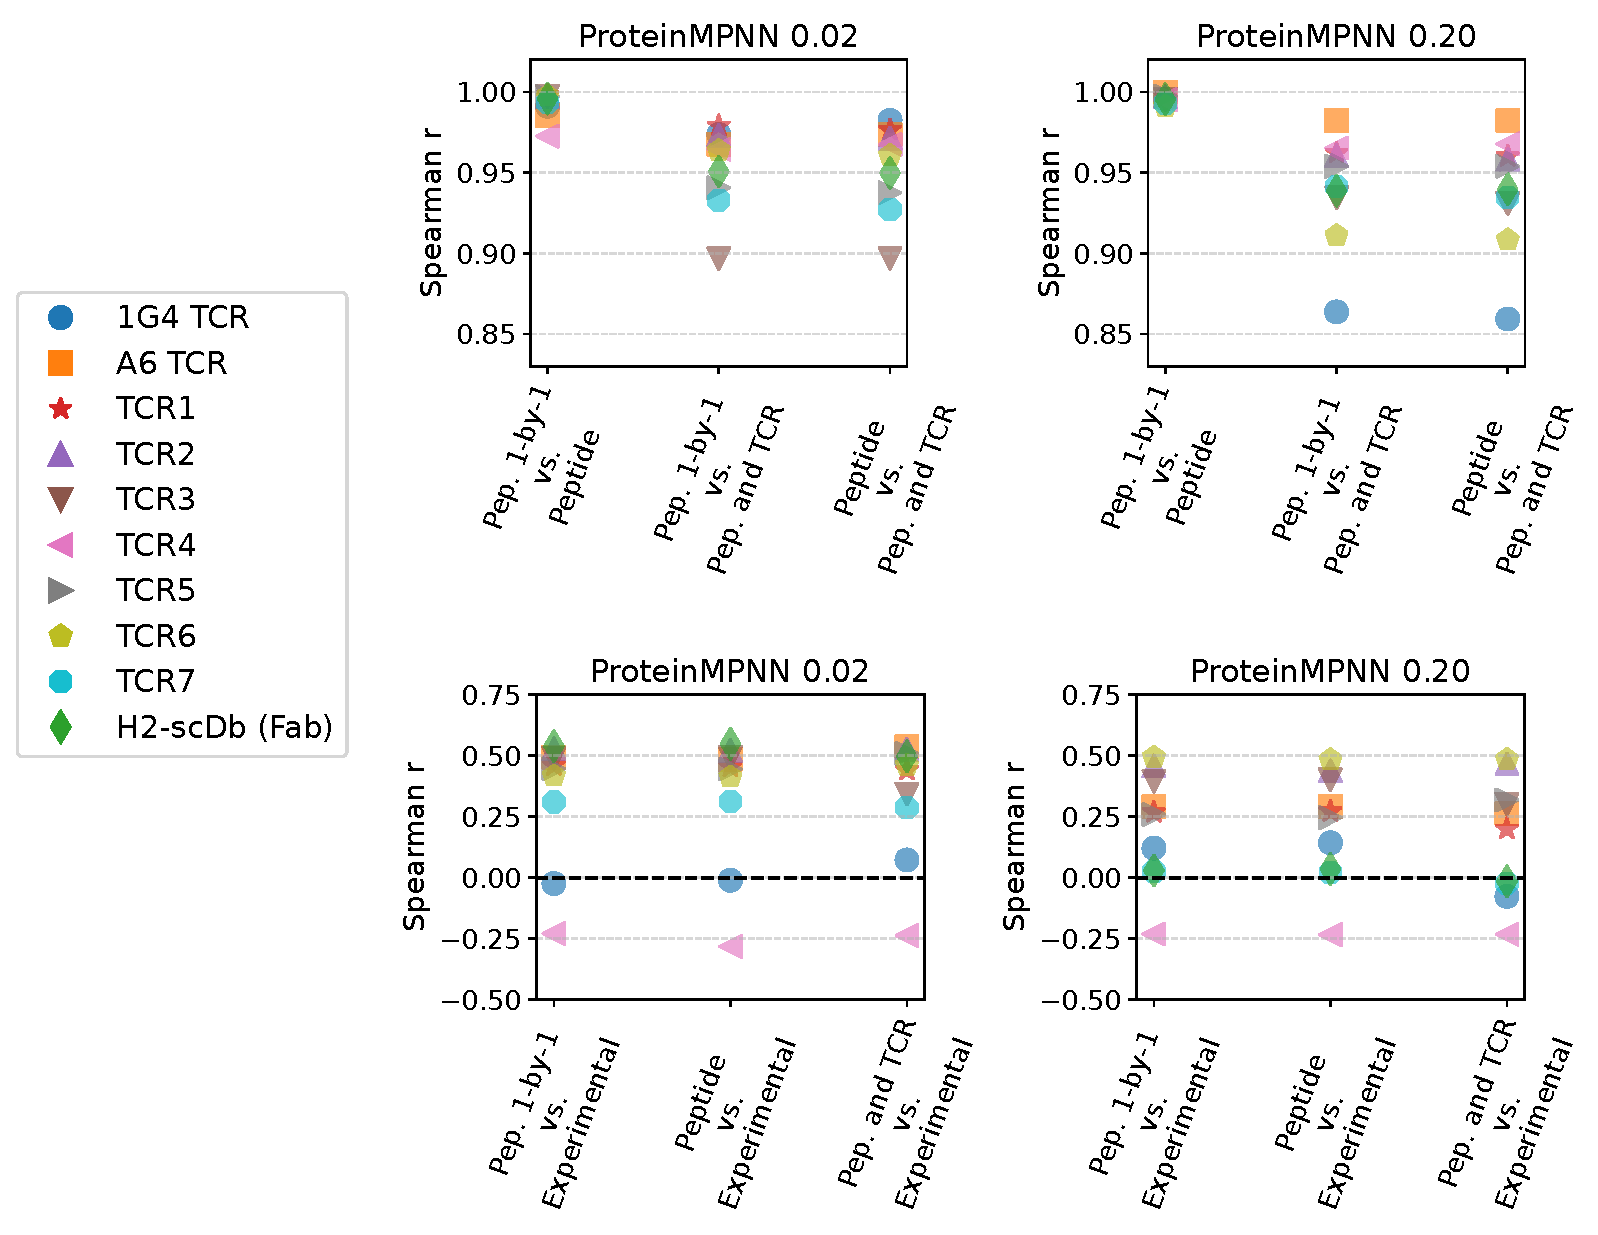
\includegraphics[width=0.90\textwidth]{figures/proteinmpnn_scoring_schemes_comparison.pdf}
\figcaption{Robustness of ProteinMPNN performance across scoring schemes .}{ The performance of
ProteinMPNN across different systems (legend) is shown for models trained with varying noise
amplitudes (specified above each panel), and using different scoring schemes. We consider three
scoring schemes: (i): ``Peptide 1-by-1" in which residues within the peptide are masked and scored
one at a time, using the remainder of the TCR-pMHC complex as structural context
(eq.~\ref{eq:peplogp_proteinmpnn}), (ii) ``Peptide" scheme, in which the entire peptide is masked
and scored simultaneously (eq.~\ref{eq:peplogp_proteinmpnn_pep}), and (iii) ``Pep. and TCR" scheme
in which both the peptide and the nearby TCR residues are masked and scored simultaneously
(eq.~\ref{eq:peplogp_proteinmpnn_tcr_and_pep}).
Top panels show the Spearman correlation between predictions from different scoring schemes, while
bottom panels show correlations between each scheme and experimental data. Results demonstrate that
ProteinMPNN predictions are robust to the choice of scoring scheme.

}
\label{fig:proteinmpnn_scoring_schemes_comparison}
\end{figure}




\begin{figure}[ht]
\centering
	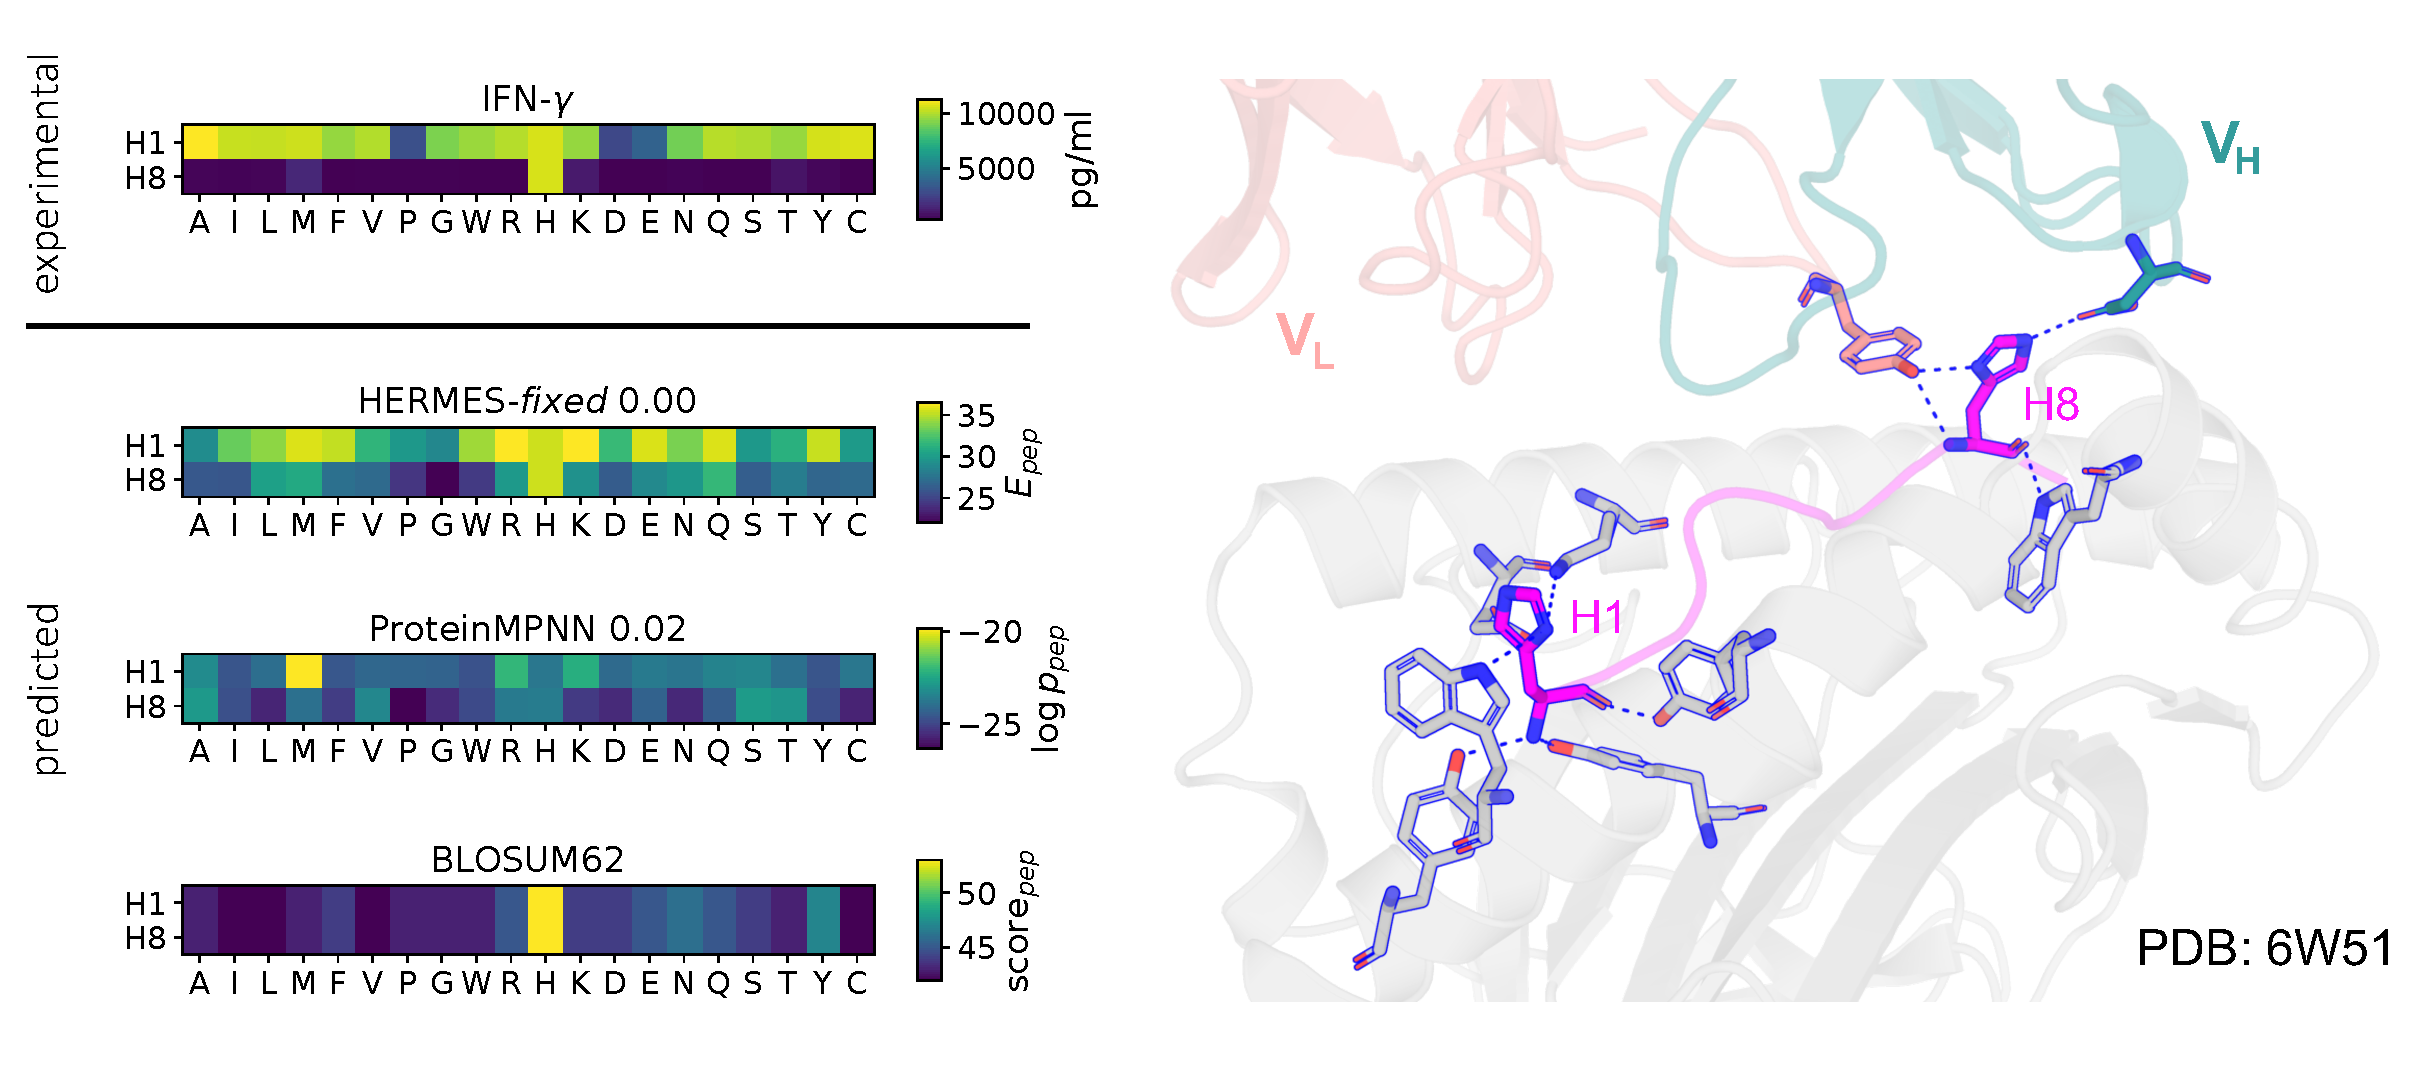
\includegraphics[width=0.8\textwidth]{figures/hsiue_h1_h8.pdf}
\figcaption{Context-dependent mutational effects on T-cell activity.}{ The heatmaps show both
experimental measurements and model predictions of T-cell activities of amino acid variants at
positions 1 and 8 of the p53$^R157H$ peptide, which we study in complex with the designed
bi-specific antibody H2-scDB and HLA-A*02:01~\cite{Hsiue2021-ag}. The wild-type peptide has a
histidine at both sites. A standard substitution matrix (such as BLOSUM62) would assign identical
scores to mutations at these two sites, because they share the same wild-type residue. However,
peptide binding and the subsequent T-cell activity depends on the structural context of each
substitution. Here, H1 forms polar contacts only with the MHC (from the sides), while H8 is more
tightly constrained by polar contacts with the TCR (right panel). HERMES-{\em fixed} correctly
leverages structural context to predict T-cell activity as a result of substitutions away from
histidines at both positions. Although ProteinMPNN also incorporates structural information, its
predictions are not as accurate in this instance.}
\label{fig:hsiue_h1_h8}
\end{figure}



\begin{figure}[ht]
\centering
	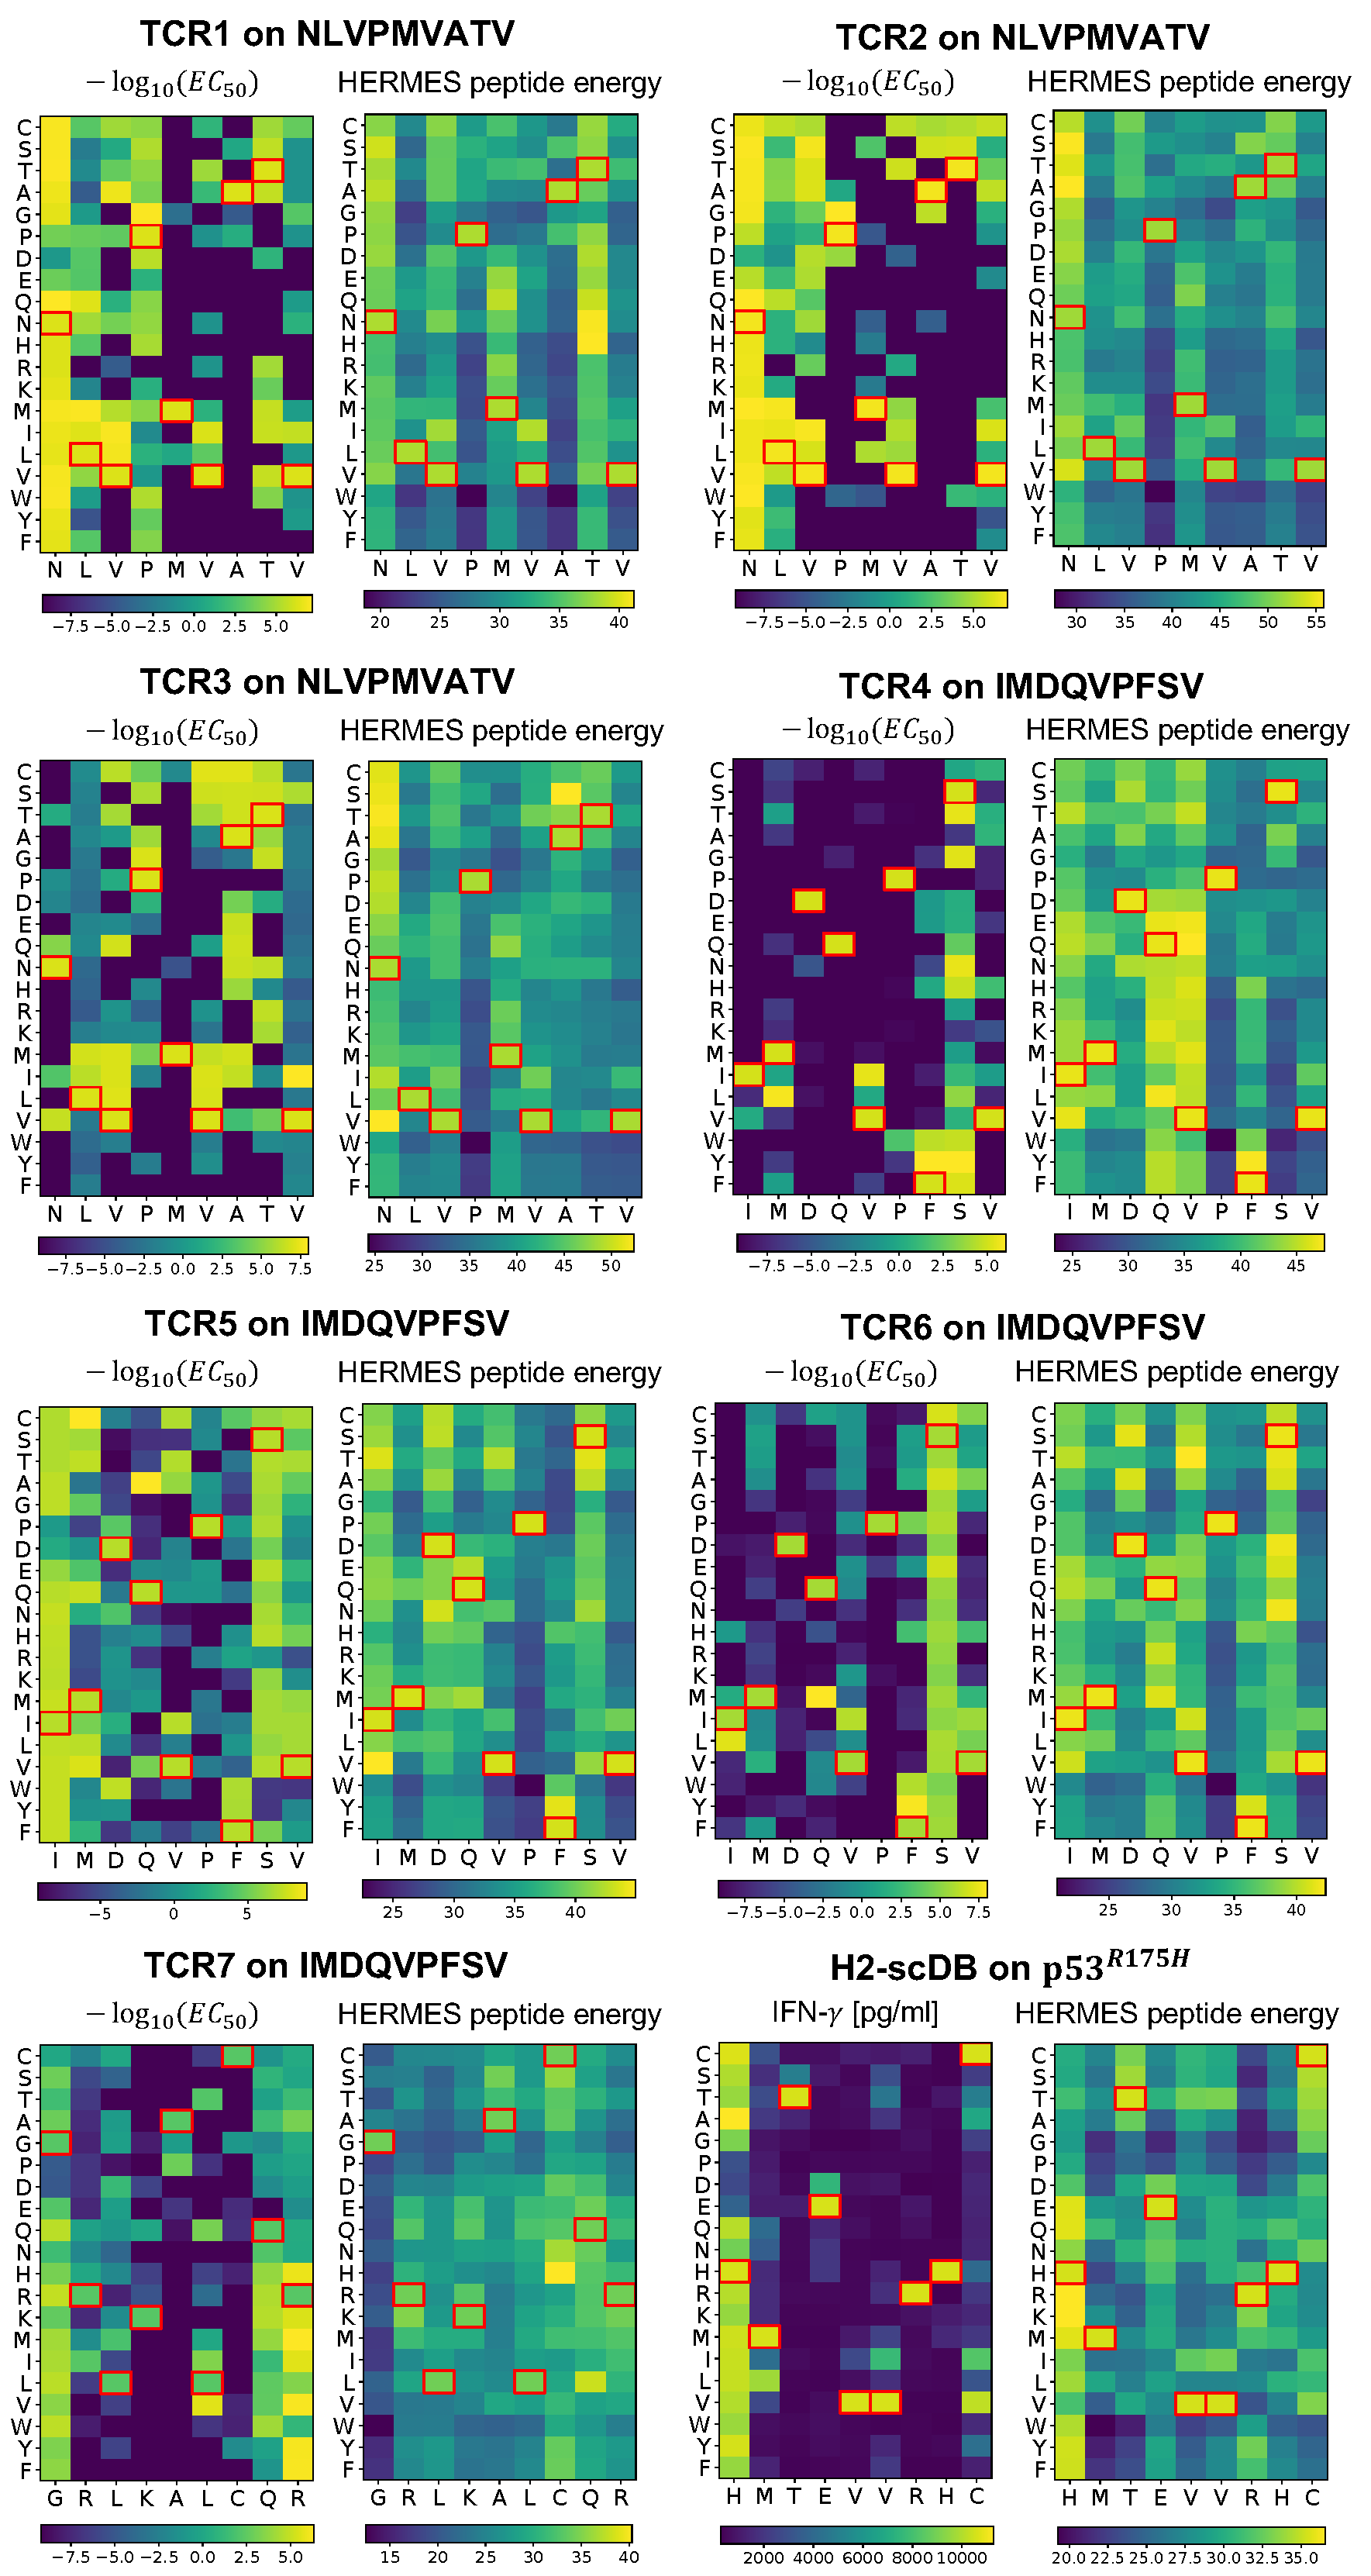
\includegraphics[width=0.63\textwidth]{figures/activity_heatmaps.pdf}
\figcaption{Mutational effect on T-cell activities}{. The heatmaps show the experimental
measurements and the predictions from the HERMES-{\em fixed} model for the effect of all single
point mutations on peptides interacting with TCR1-7~\cite{Luksza2022-gx}, and the designed
bi-specific antibody Fab in the H2-scDB system~\cite{Hsiue2021-ag} (similar to the data presented in
scatter plots in Fig.~3). In the heatmaps, each column corresponds to a position in the peptide and
is labeled with its wild-type amino acid (indicated by a red square on the heatmaps), and the rows
show the amino acid substitutions. }
\label{fig:activity_heatmaps}
\end{figure}




\begin{figure}[ht]
\centering
	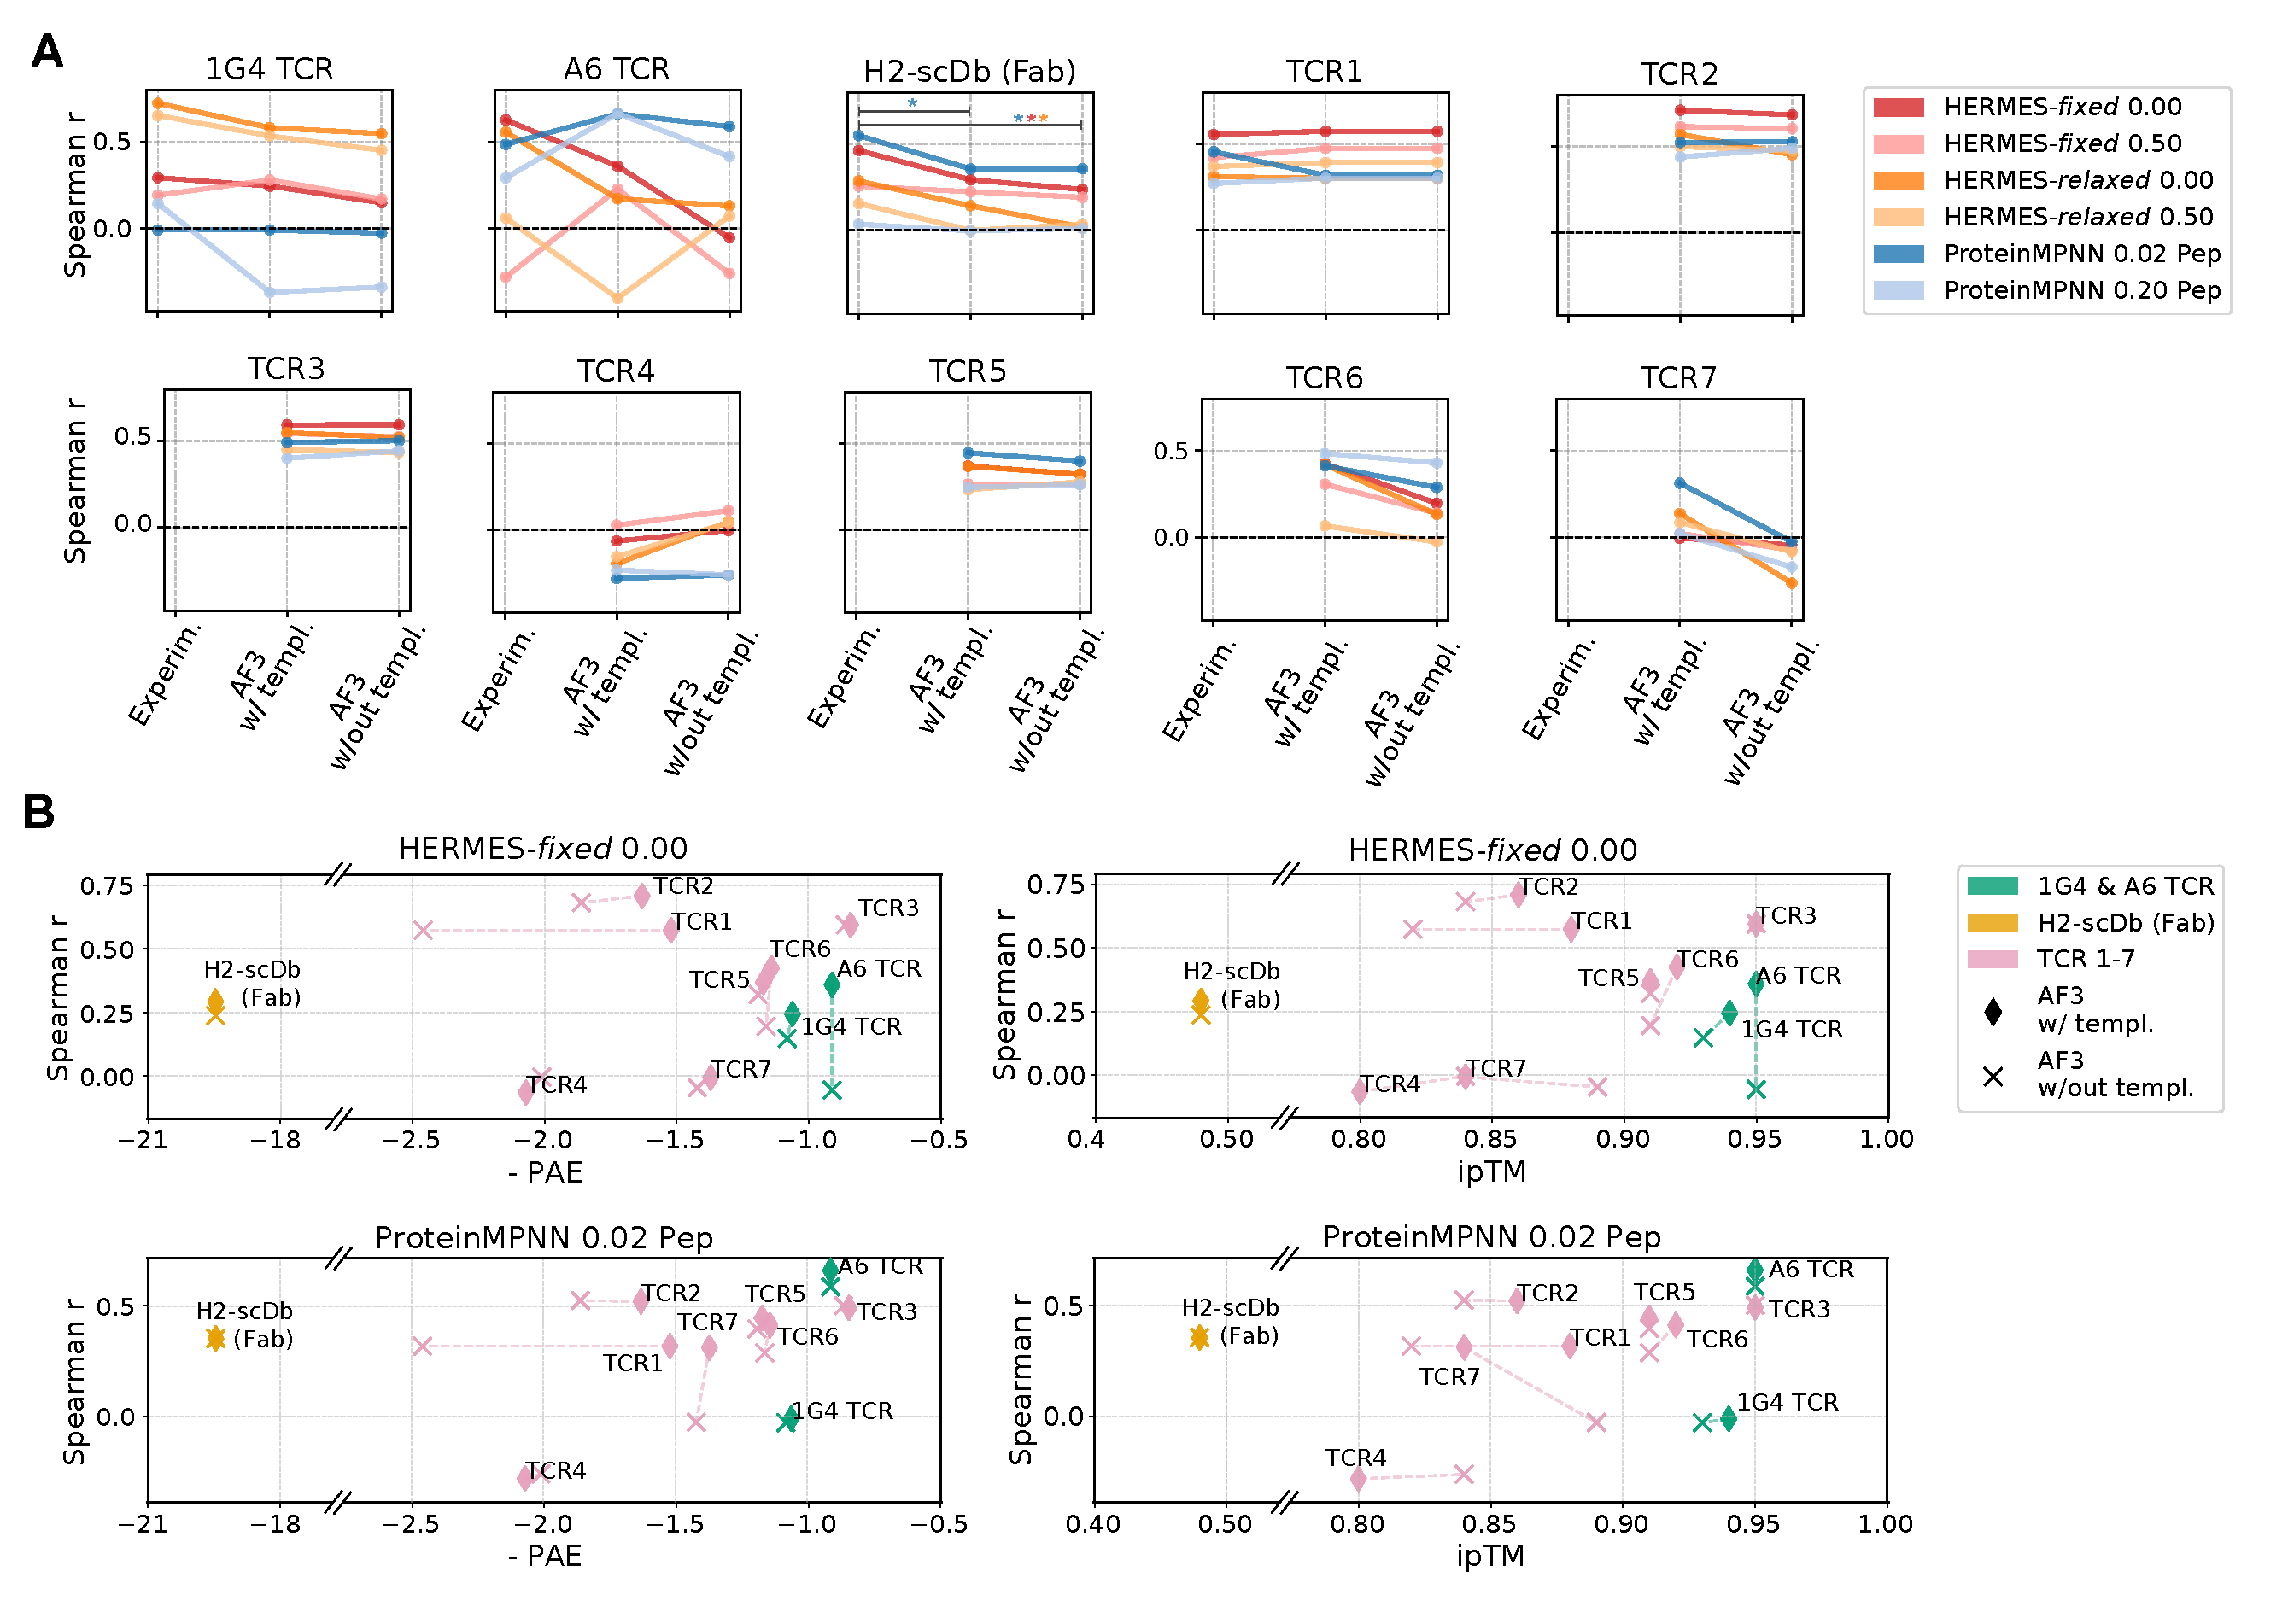
\includegraphics[width=\textwidth]{figures/plots_af3_struc_ablation.pdf}
\figcaption{
 HERMES and ProteinMPNN prediction accuracies for AlphaFold3-predicted structures.}{ {\bf (A)} For
 all systems analyzed, we used the AlphaFold Server to model the structures of complexes with the
 wild-type peptides, both with and without template guidance; see
 Table~\ref{table:af3_folding_metrics} for details on the confidence of these AF3 models. For each
 system, the Spearman correlation ($r$) between experimental affinity or activity data and
 predictions from HERMES and ProteinMPNN models (colors) is shown for three structure inputs:
 experimental structures (when available), AF3 model with template, and AF3 model without template.
Statistically significant drop in accuracy between models using experimental vs. AF3
structures--defined as cases with p-value$<0.05$ for difference in the Fisher's $z$-transformed
Spearman correlations--are indicated with an asterisk (*) in the same color as that of the model
(from the legend). Such drops are only observed for the H2-scDb Fab-pMHC system, where AF3 failed to
generate a realistic structure. {\bf (B)} Spearman correlation ($r$) between experimental
affinity/activity data and predictions from the overall best HERMES-{\em fixed} (top) and
ProteinMPNN (bottom) models from (A), plotted against AF3 confidence metrics: negative predicted
alignment error ($-$PAE; left) and interchain predicted TM-score (ipTM; right). Results are shown
for AF3 structures generated with and without template guidance. The confidence metrics are reported
in Table~\ref{table:af3_folding_metrics}.
 The HERMES model names specify the scoring scheme (fixed, relaxed), and the noise amplitude (in
 \AA) injected to the coordinates of the structure data during training. Similarly, the ProteinMPNN
 model names capture scoring scheme, i.e., the whole peptide (eq.~\ref{eq:peplogp_proteinmpnn_pep}),
 and the noise amplitude injected to the training data.
}
\label{fig:plots_af3_struc_ablation}
\end{figure}







\begin{figure}[ht]
\centering
	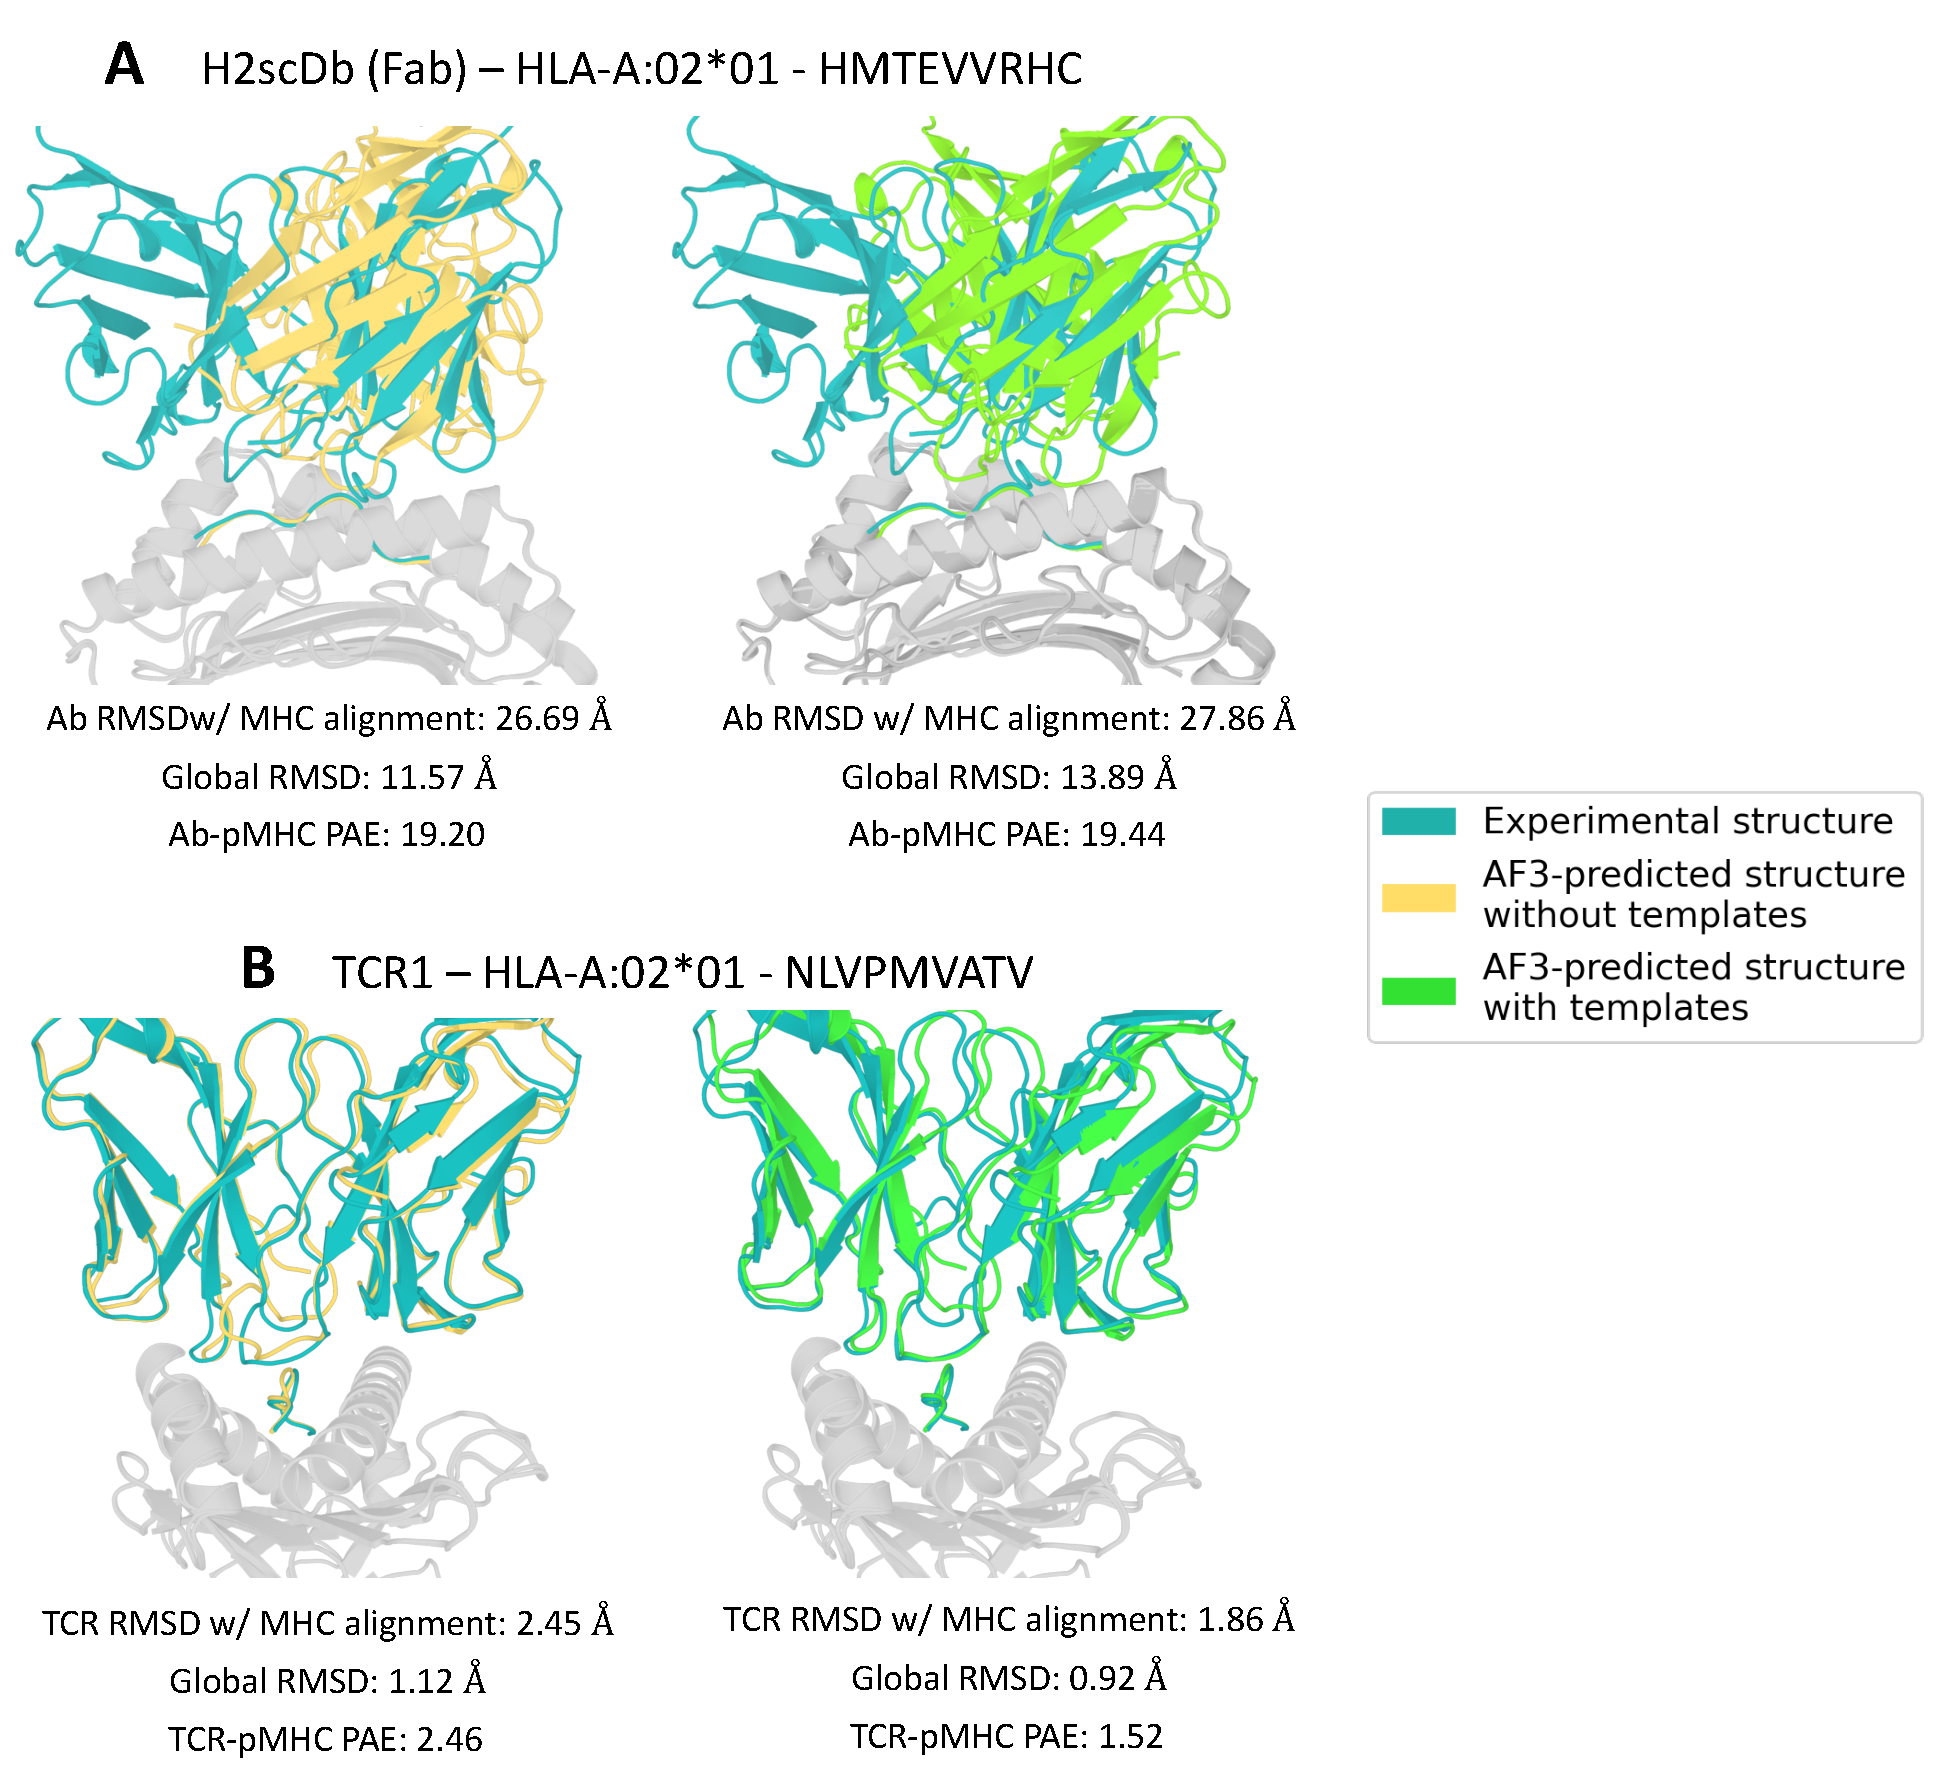
\includegraphics[width=0.8\textwidth]{figures/af3_folded_structures_example.pdf}
\figcaption{Comparison of experimentally determined structures with AlphaFold3 predicted
structures.}{
The experimentally determined structure of {\bf (A)} H2-scDb Fab-pMHC complex, and {\bf (B)}
TCR1-pMHC complex are
shown against the AF3 predicted structures generated without (left) and with (right) template
guidance. All structures were aligned on the MHC using PyMOL to enable consistent visualiziation of
TCR/Fab docking geometries. AF3 failed to produce a realistic structure model for the H2-scDb
system, as evidenced by the high RMSD and interface PAE values reported in
Table~\ref{table:af3_folding_metrics}.
}
\label{fig:af3_folded_structures_example}
\end{figure}





\begin{figure}[ht]
\centering
	\includegraphics[width=0.95\textwidth]{figures/joint_design_distributions_2.pdf}
\figcaption{Peptide design energy profiles across systems and HERMES models.}{
For the NY-ESO system, panels {\bf (A)} and {\bf (B)} show the distribution of peptide energies
(eq.~\ref{eq:pepEn}) divided by the length, for peptides designed with HERMES-{\em fixed} and
HERMES-{\em relaxed} protocols, respectively.
Designs were pooled across the two structure templates used (2BNQ and 2BNR), with the peptide
energies computed using their respective template structures. In all panels, the red lines indicates
the energies of the wild-type peptides in their corresponding structures. {\bf(C)} The scaled energy
of the designed peptides are shown as a function of the MCMC iterations during the HERMES-{\em
relaxed} protocol, using the two different structural templates for the NY-ESO system: 2BNQ (top)
and 2BNR (bottom). The red line indicates the energy of the wild-type peptide in its respective
structure. In panels (A-C), designs are grouped by the noise amplitude applied during HERMES
training (no noise: 0.00\AA, and moderate noise: 0.50\AA), as indicated above each panel. The
HERMES-{\em relaxed} protocol consistently produces peptides with more favorable (higher) peptide
energies than that of the wild-type, indicating that the protocol can successfully optimize within
the peptide energy landscapes; models trained with noise are more successful in finding peptides
with higher energy values.
Panels {\bf (D-F)} and {\bf (G-I)} present analogous design statistics for the EBV and the MAGE
systems, respectively.}
\label{fig:joint_design_distributions}
\end{figure}




\begin{figure}[ht]
\centering
	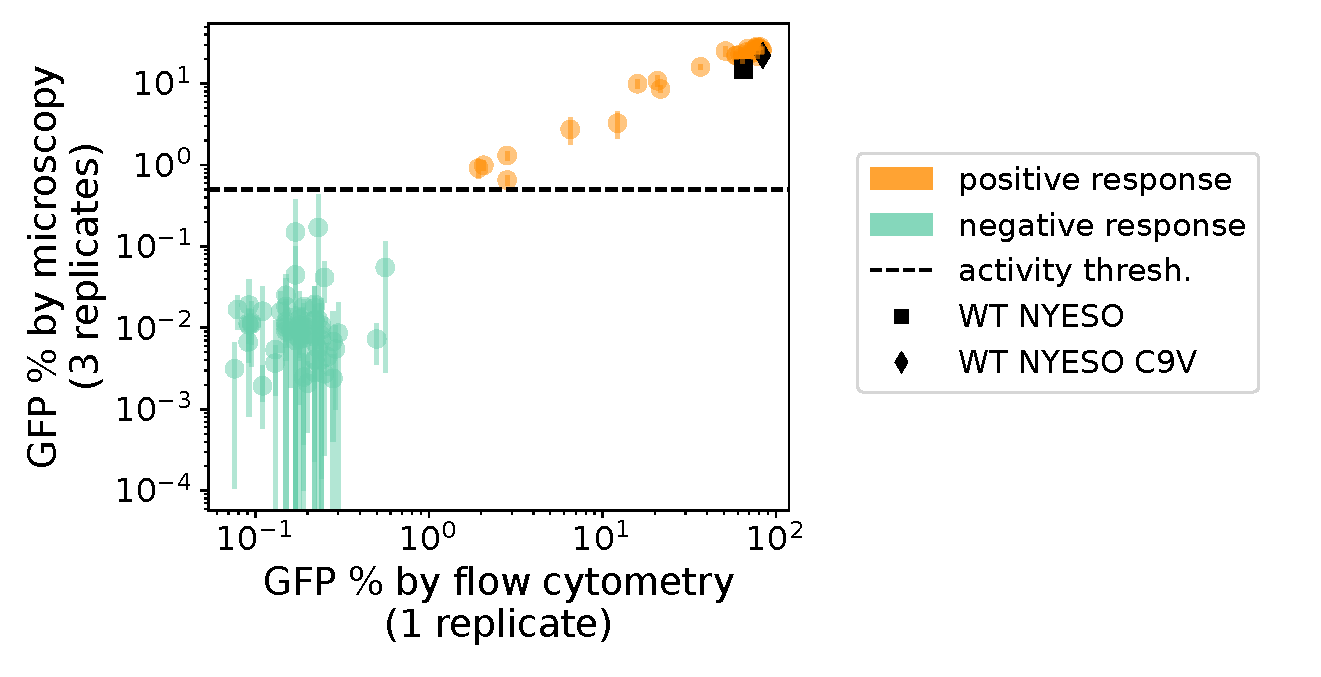
\includegraphics[width=0.7\textwidth]{figures/flow_vs_microscopy.pdf}
\figcaption{Measurements of GFP levels by flow cytometry and fluorescence microscopy.}{ For the
NY-ESO system, we performed measurements of GFP levels from peptide-induced T-cell activities, using
both flow cytometry and fluorescence microscopy. Fluorescence microscopy measurements were performed
in three independent replicates; markers denote the mean GFP level, and error bars show the standard
deviation across the three replicates. Flow cytometry was done only on a single replicate.
The two measurement methods demonstrate good agreement, with a clear separation between designs that
induced significant T-cell activation (orange) and those that did not (green). The black markers
indicate the activities induced by the wild-type peptides.
}
\label{fig:flow_vs_microscopy}
\end{figure}




\begin{figure}[ht]
\centering
	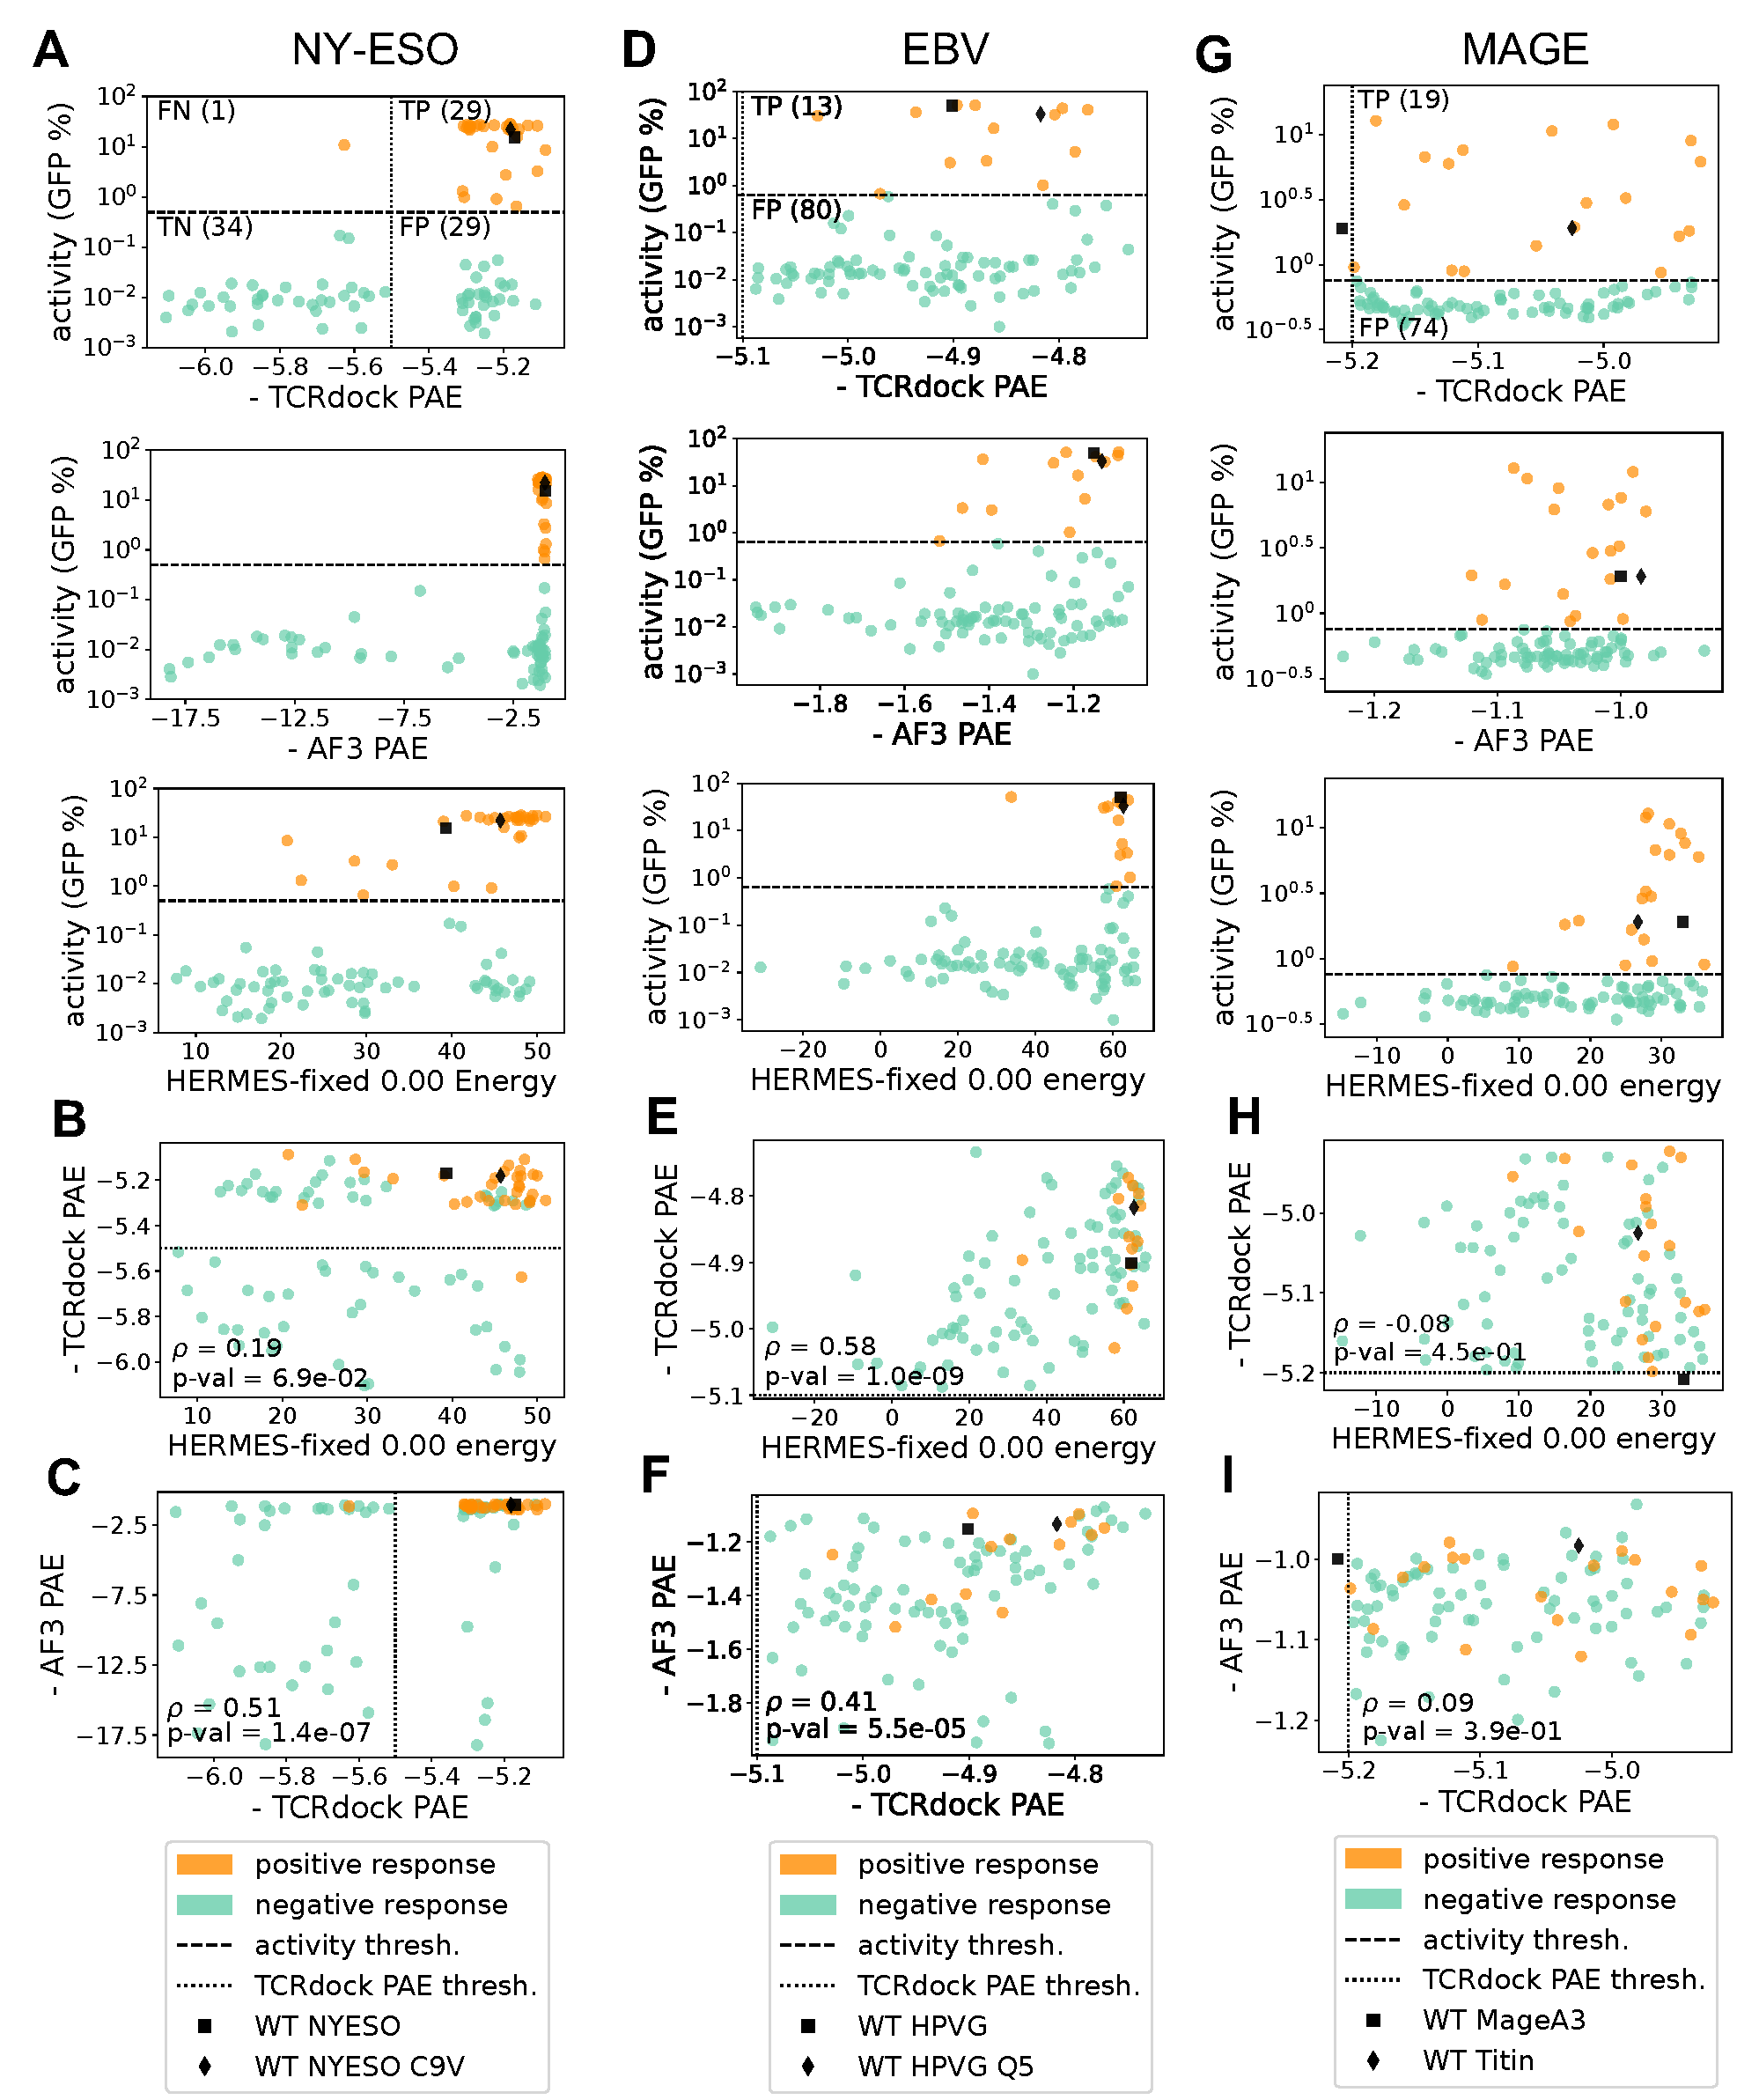
\includegraphics[width=0.90\textwidth]{figures/design_scatterplots.pdf}
\figcaption{TCRdock and AlphaFold3 PAEs for HERMES-designed peptides}{. {\bf(A)} For the NY-ESO
system, the induced T-cell activity by the designed peptides is shown against the computed TCRdock
negative-PAE (first row), the AlphaFold3 negative-PAE (second row), and the energy score predicted
with HERMES-{\em fixed} 0.00 (non noise during training) (third row); higher negative-PAE's indicate
better designs. For the designed peptides in the NY-ESO system {\bf(B)} shows the relationship
between negative TCRdock PAE values and the peptide energies from the HERMES-{\em fixed} 0.00.
model, and {\bf (C)} shows the negative AlphaFold3 PAE versus TCRdock PAE values. Peptides that
induced significant T-cell responses are shown in orange, and non-responders are shown in green. The
vertical dashed line indicate the filtering threshold for TCRdock PAE, with points to the right
representing the negative design set. Panels {\bf (D-F)} and {\bf (G-I)} show analogous statistics
for the EBV and the MAGE system, respectively. No negative designs (i.e., designs below the
respective TCRdock negative-PAE thresholds) were experimentally validated for these systems. We
observe that the HERMES scores and TCRdock PAE values are uncorrelated or only weakly correlated
across systems, and so are TCRdock and AF3 PAE, suggesting that AF3 and TCRdock PAE's can serve as
complementary filters to HERMES during design.
}
\label{fig:design_scatterplots}
\end{figure}



\begin{figure}[ht]
\centering
	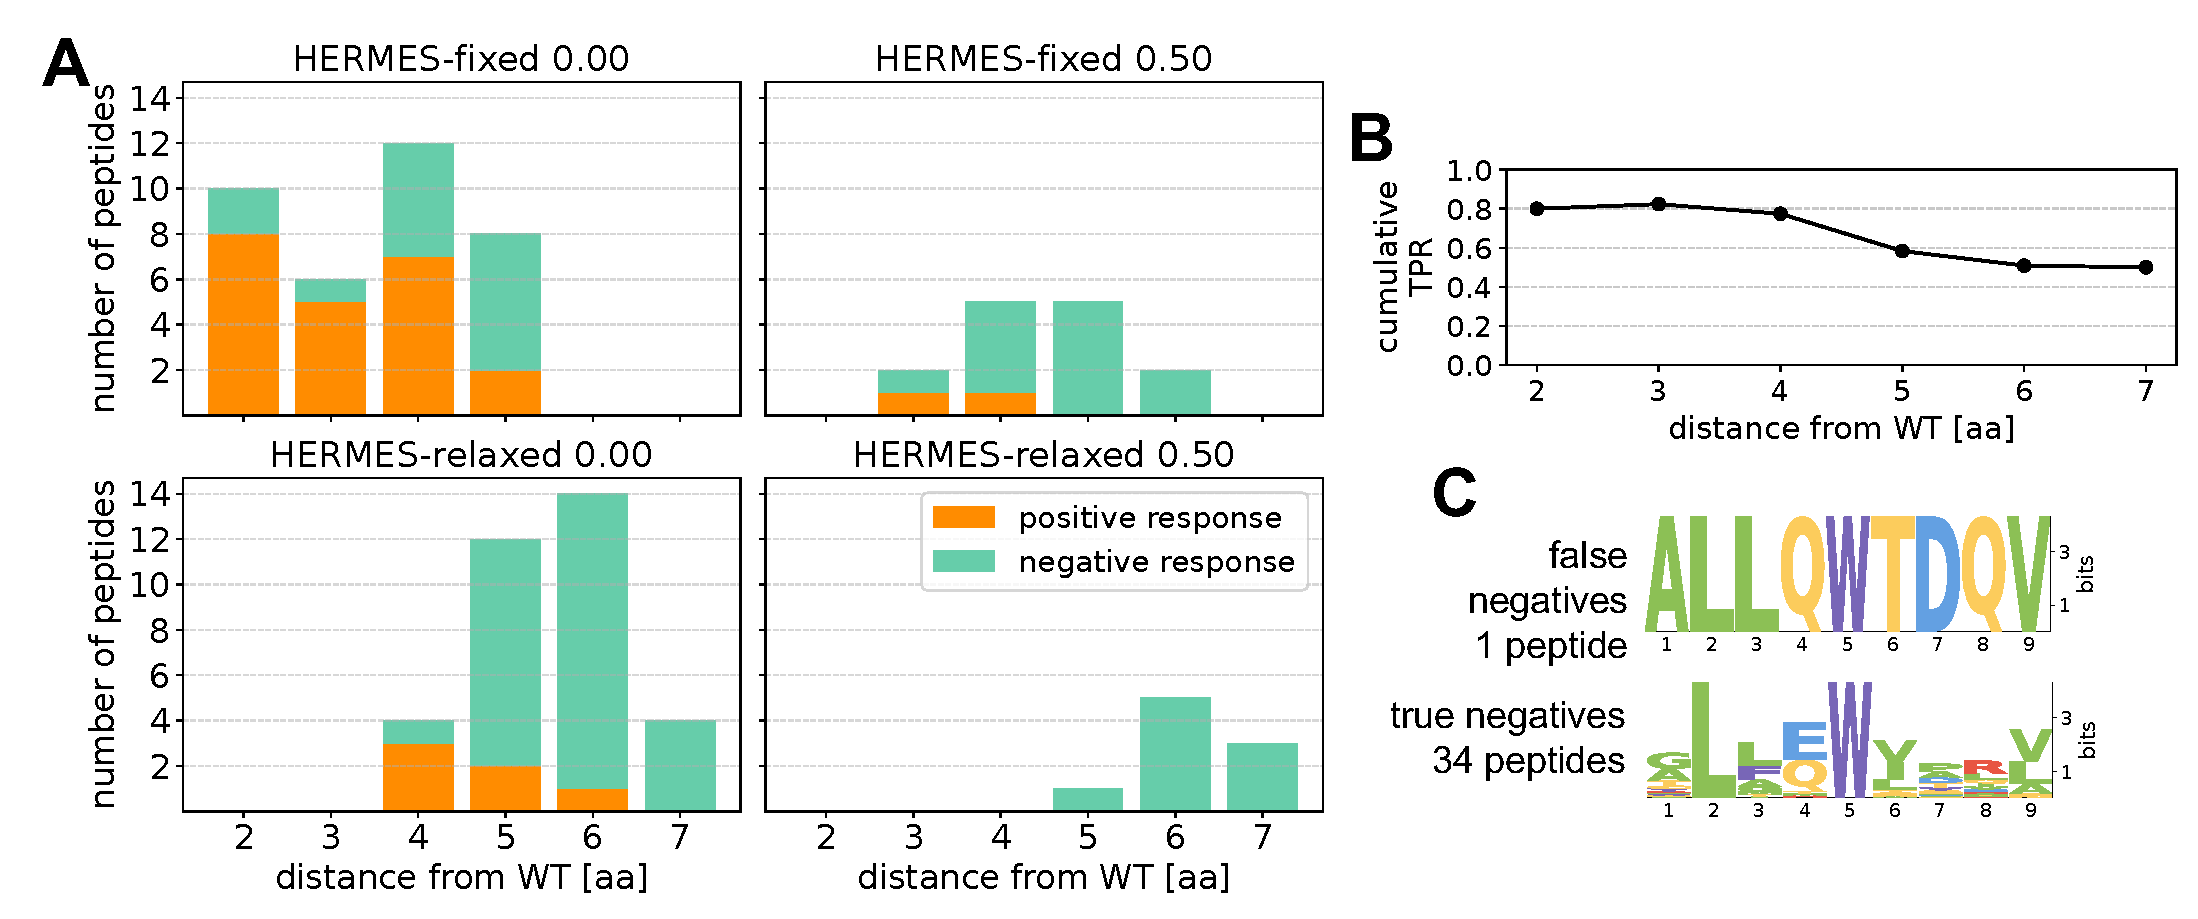
\includegraphics[width=0.99\textwidth]{figures/design_experimental_nyeso.pdf}
\figcaption{Experimental T-cell activation by HERMES-designed peptides in the NY-ESO system}{. {\bf
(A)} The number of peptides designed by different HERMES models (panels) that induced GFP expression
beyond the T-cell activation threshold (positives; shown in orange) versus those that did not
(negatives; shown in green) is shown. The designed peptides are grouped according to their minimum
Hamming distance from any of the wild-type sequences used as design templates
(Table~\ref{table:design_info}). The HERMES model names specify the scoring scheme (fixed, relaxed),
and the noise amplitude (in \AA) injected to the coordinates of the structure data during training.
{\bf (B)} The cumulative True Positive Rate (TPR) for designed peptides is shown as a function of
their Hamming distance from any of the wild-types. {\bf (C)} Logo plots show the sequence
composition of the False Negative and the True Negative designs. }
\label{fig:design_experimental_nyeso}
\end{figure}



\begin{figure}[ht]
\centering
	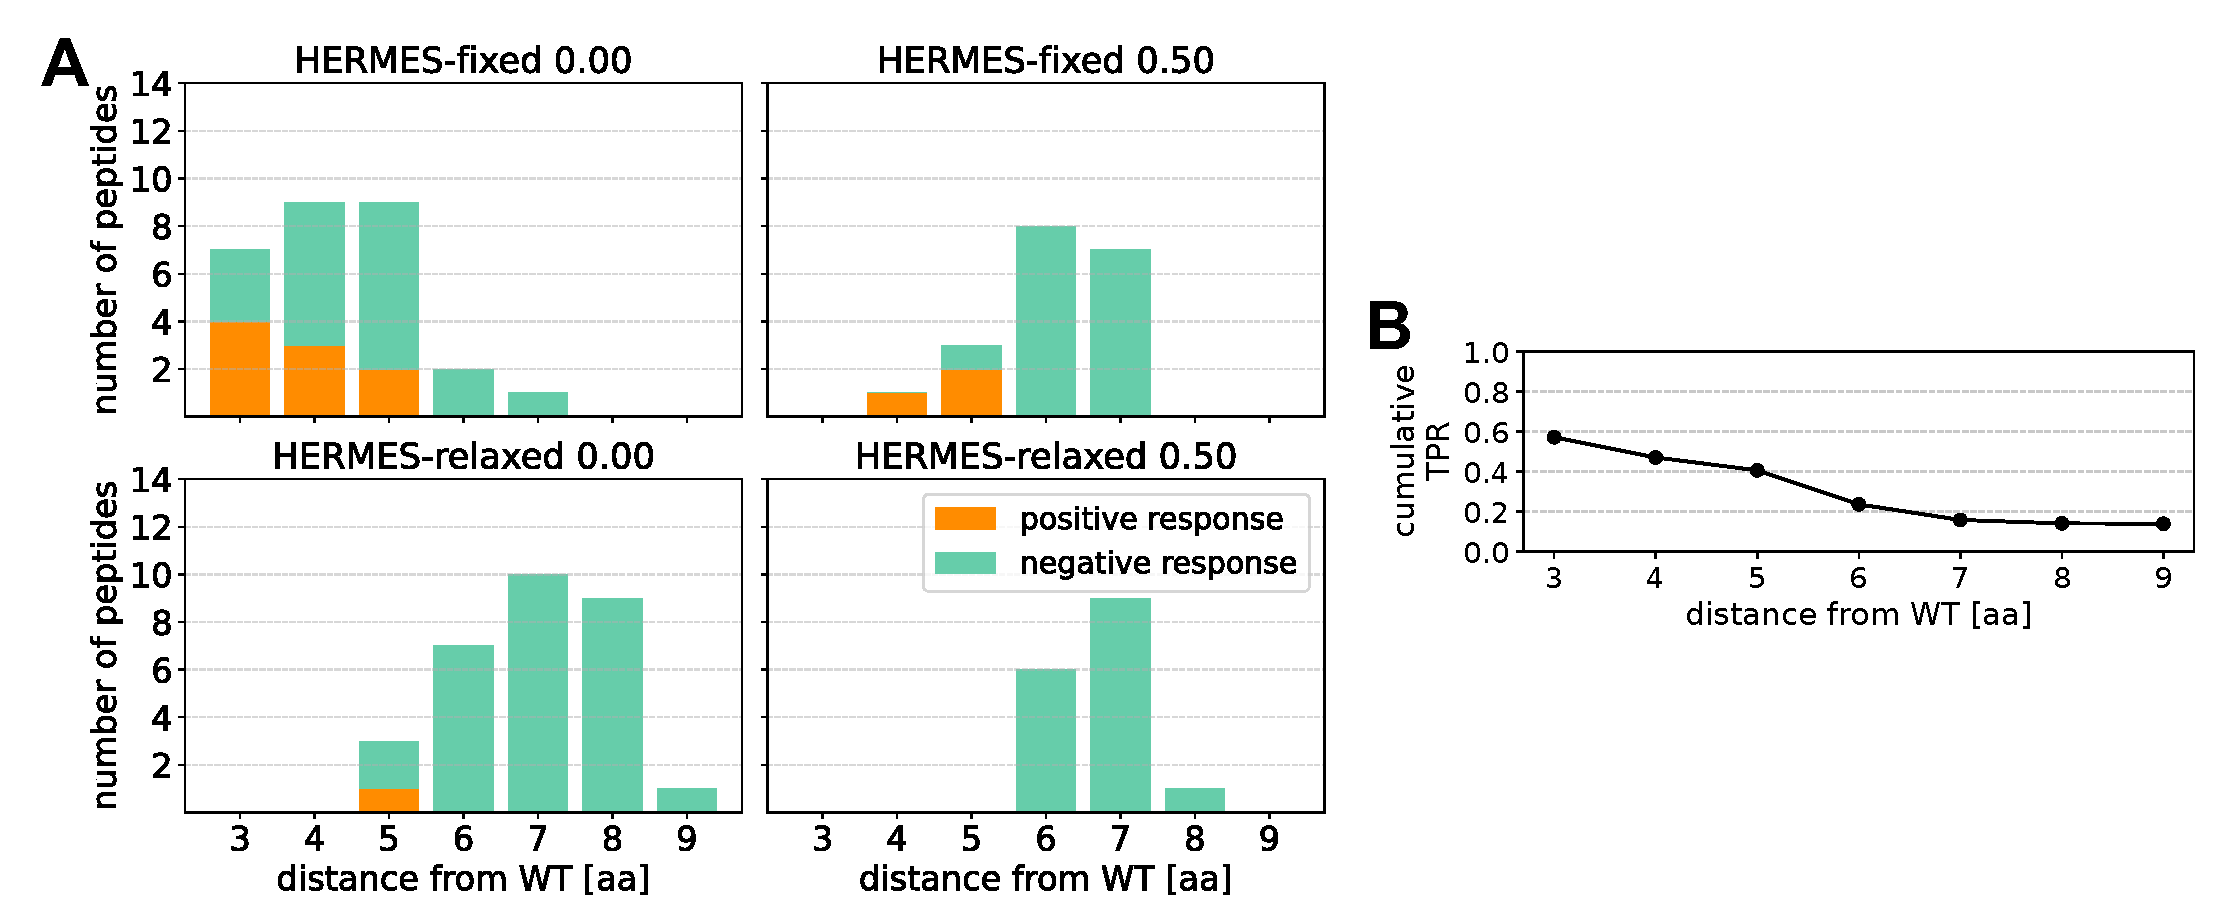
\includegraphics[width=0.99\textwidth]{figures/design_experimental_ebv.pdf}
\figcaption{Experimental T-cell activation by HERMES-designed peptides in the EBV system.}{ {\bf
(A-B)} Similar to (A-B) of Fig.~\ref{fig:design_experimental_nyeso} but for the EBV system.
}
\label{fig:design_experimental_ebv}
\end{figure}



\begin{figure}[ht]
\centering
	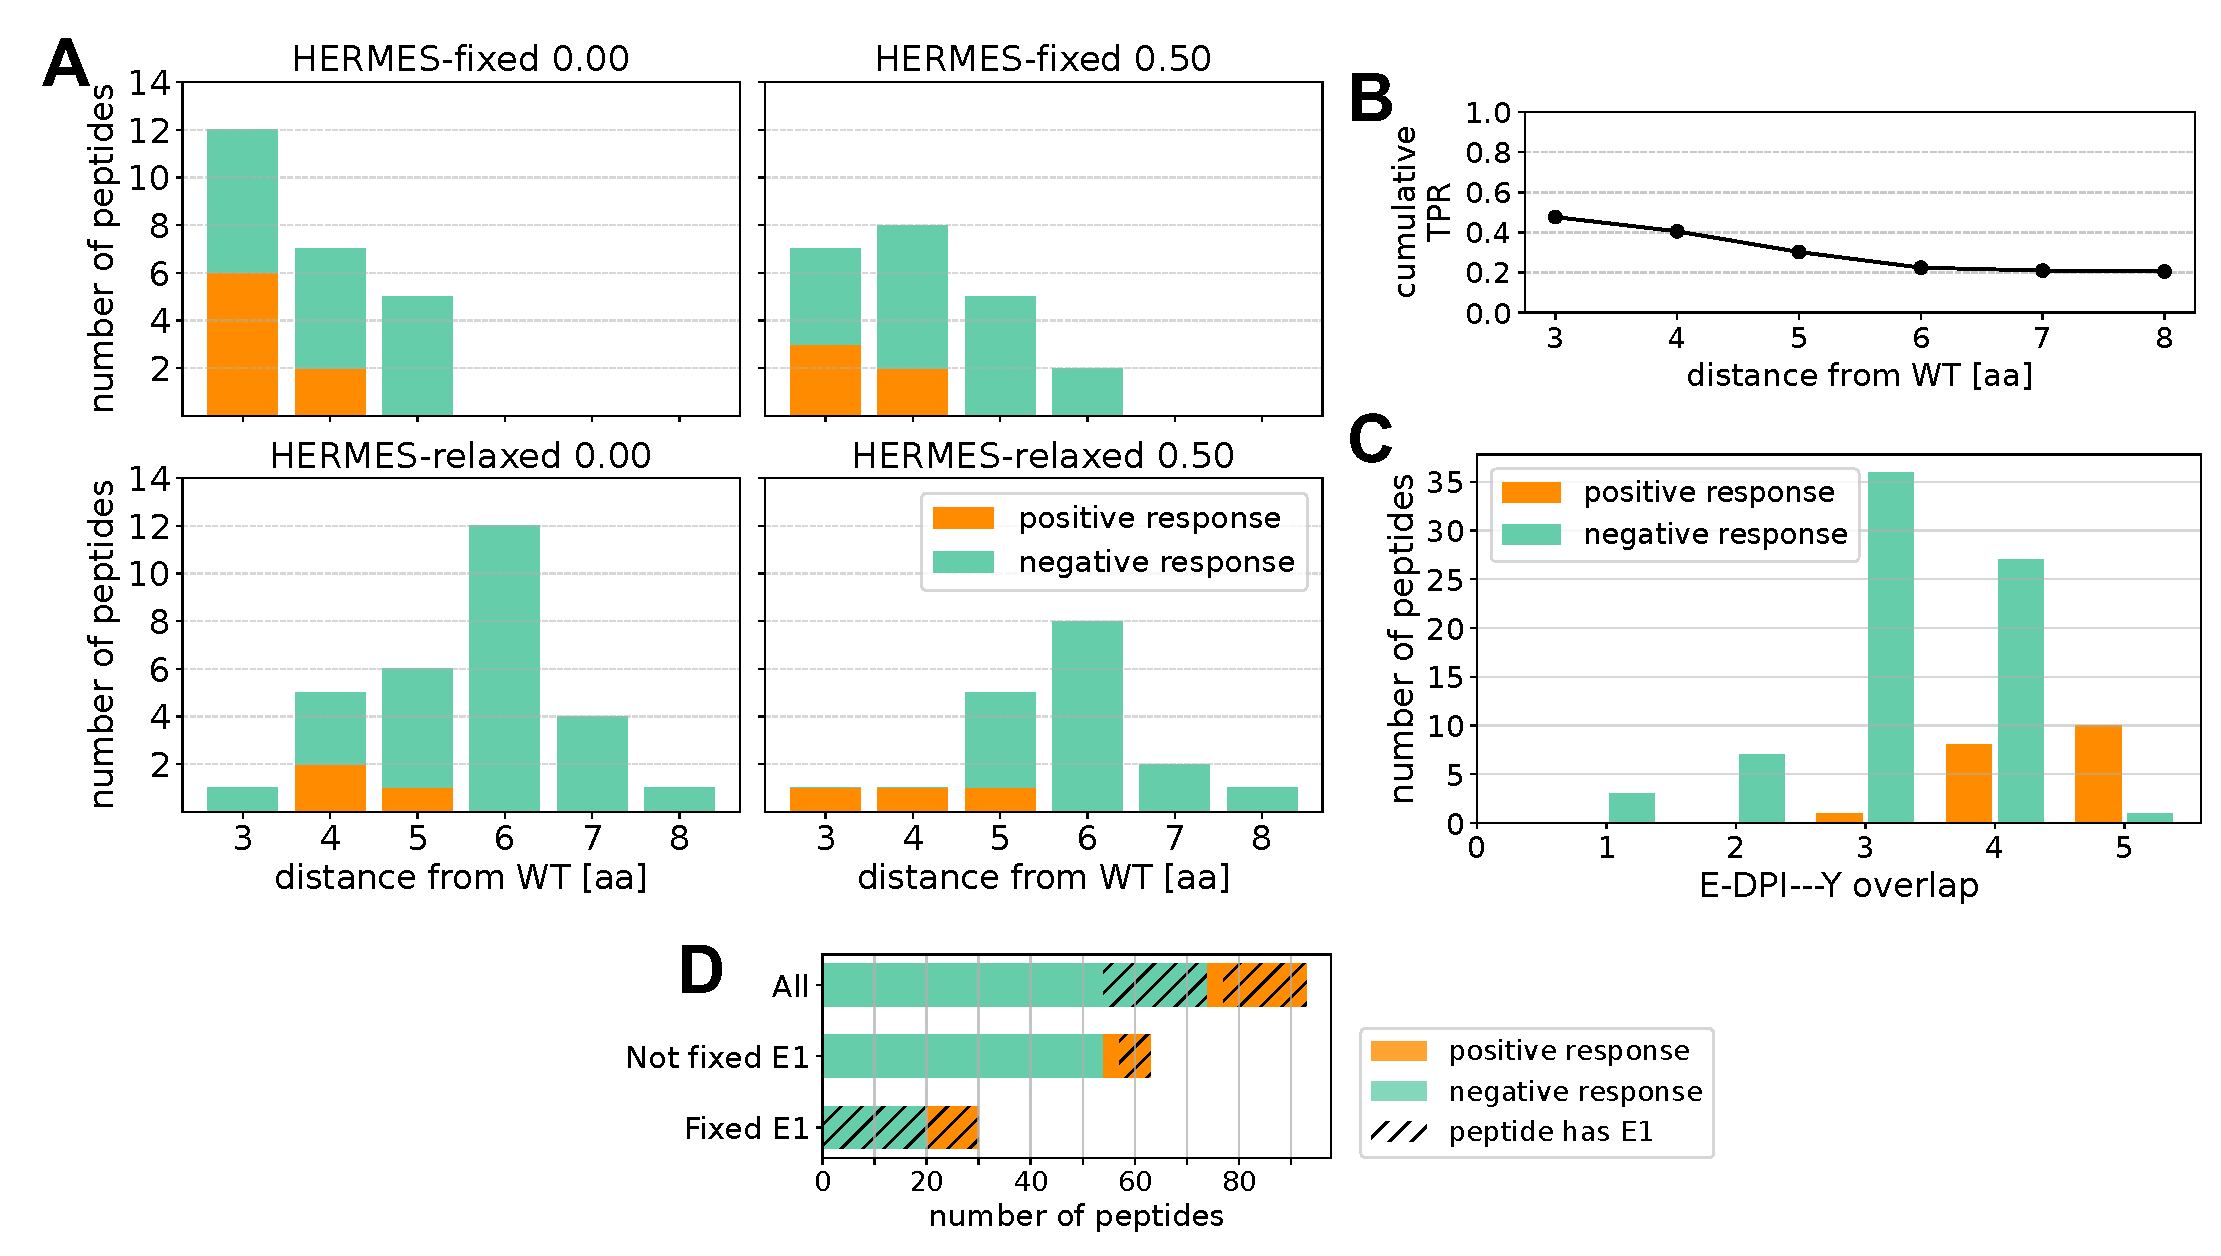
\includegraphics[width=0.99\textwidth]{figures/design_experimental_mage.pdf}
\figcaption{Experimental T-cell activation by HERMES-designed peptides in the MAGE system.}{
{\bf (A-B)} Similar to (A-B) of Fig.~\ref{fig:design_experimental_nyeso} but for the MAGE system.
\textbf{(C)} The number of designs that induced GFP expression beyond the T-cell activation
threshold (positive response; in orange) versus those that did not (negative response; in green)
 is shown as a function of the designs' overlap with the E-DPI-\,-\,-Y motif; this motif has been
 shown to enhance T-cell activation in this system~\cite{Cameron2013-vw}. The overlap is the number
 of amino acids that a design shares with the E-DPI-\,-\,-Y motif (maximum of 5). The fraction of
 positive designs increases with greater similarity to the motif. \textbf{(D)} Shown are the numbers
 of True Positives (orange) and False Positives (green) among designs generated under two protocols:
 one that enforced glutamic acid at position one (E$_1$)---labeled ``fixed E$_1$"----and one that
 did not enforce E$_1$---labeled ``not fixed E$_1$". For each protocol, the dashed segments indicate
 the number of designs that contain E$_1$. The ``All" bar presents the aggregate data from both
 protocols.
}
\label{fig:design_experimental_mage}
\end{figure}




\begin{figure}[ht]
\centering
	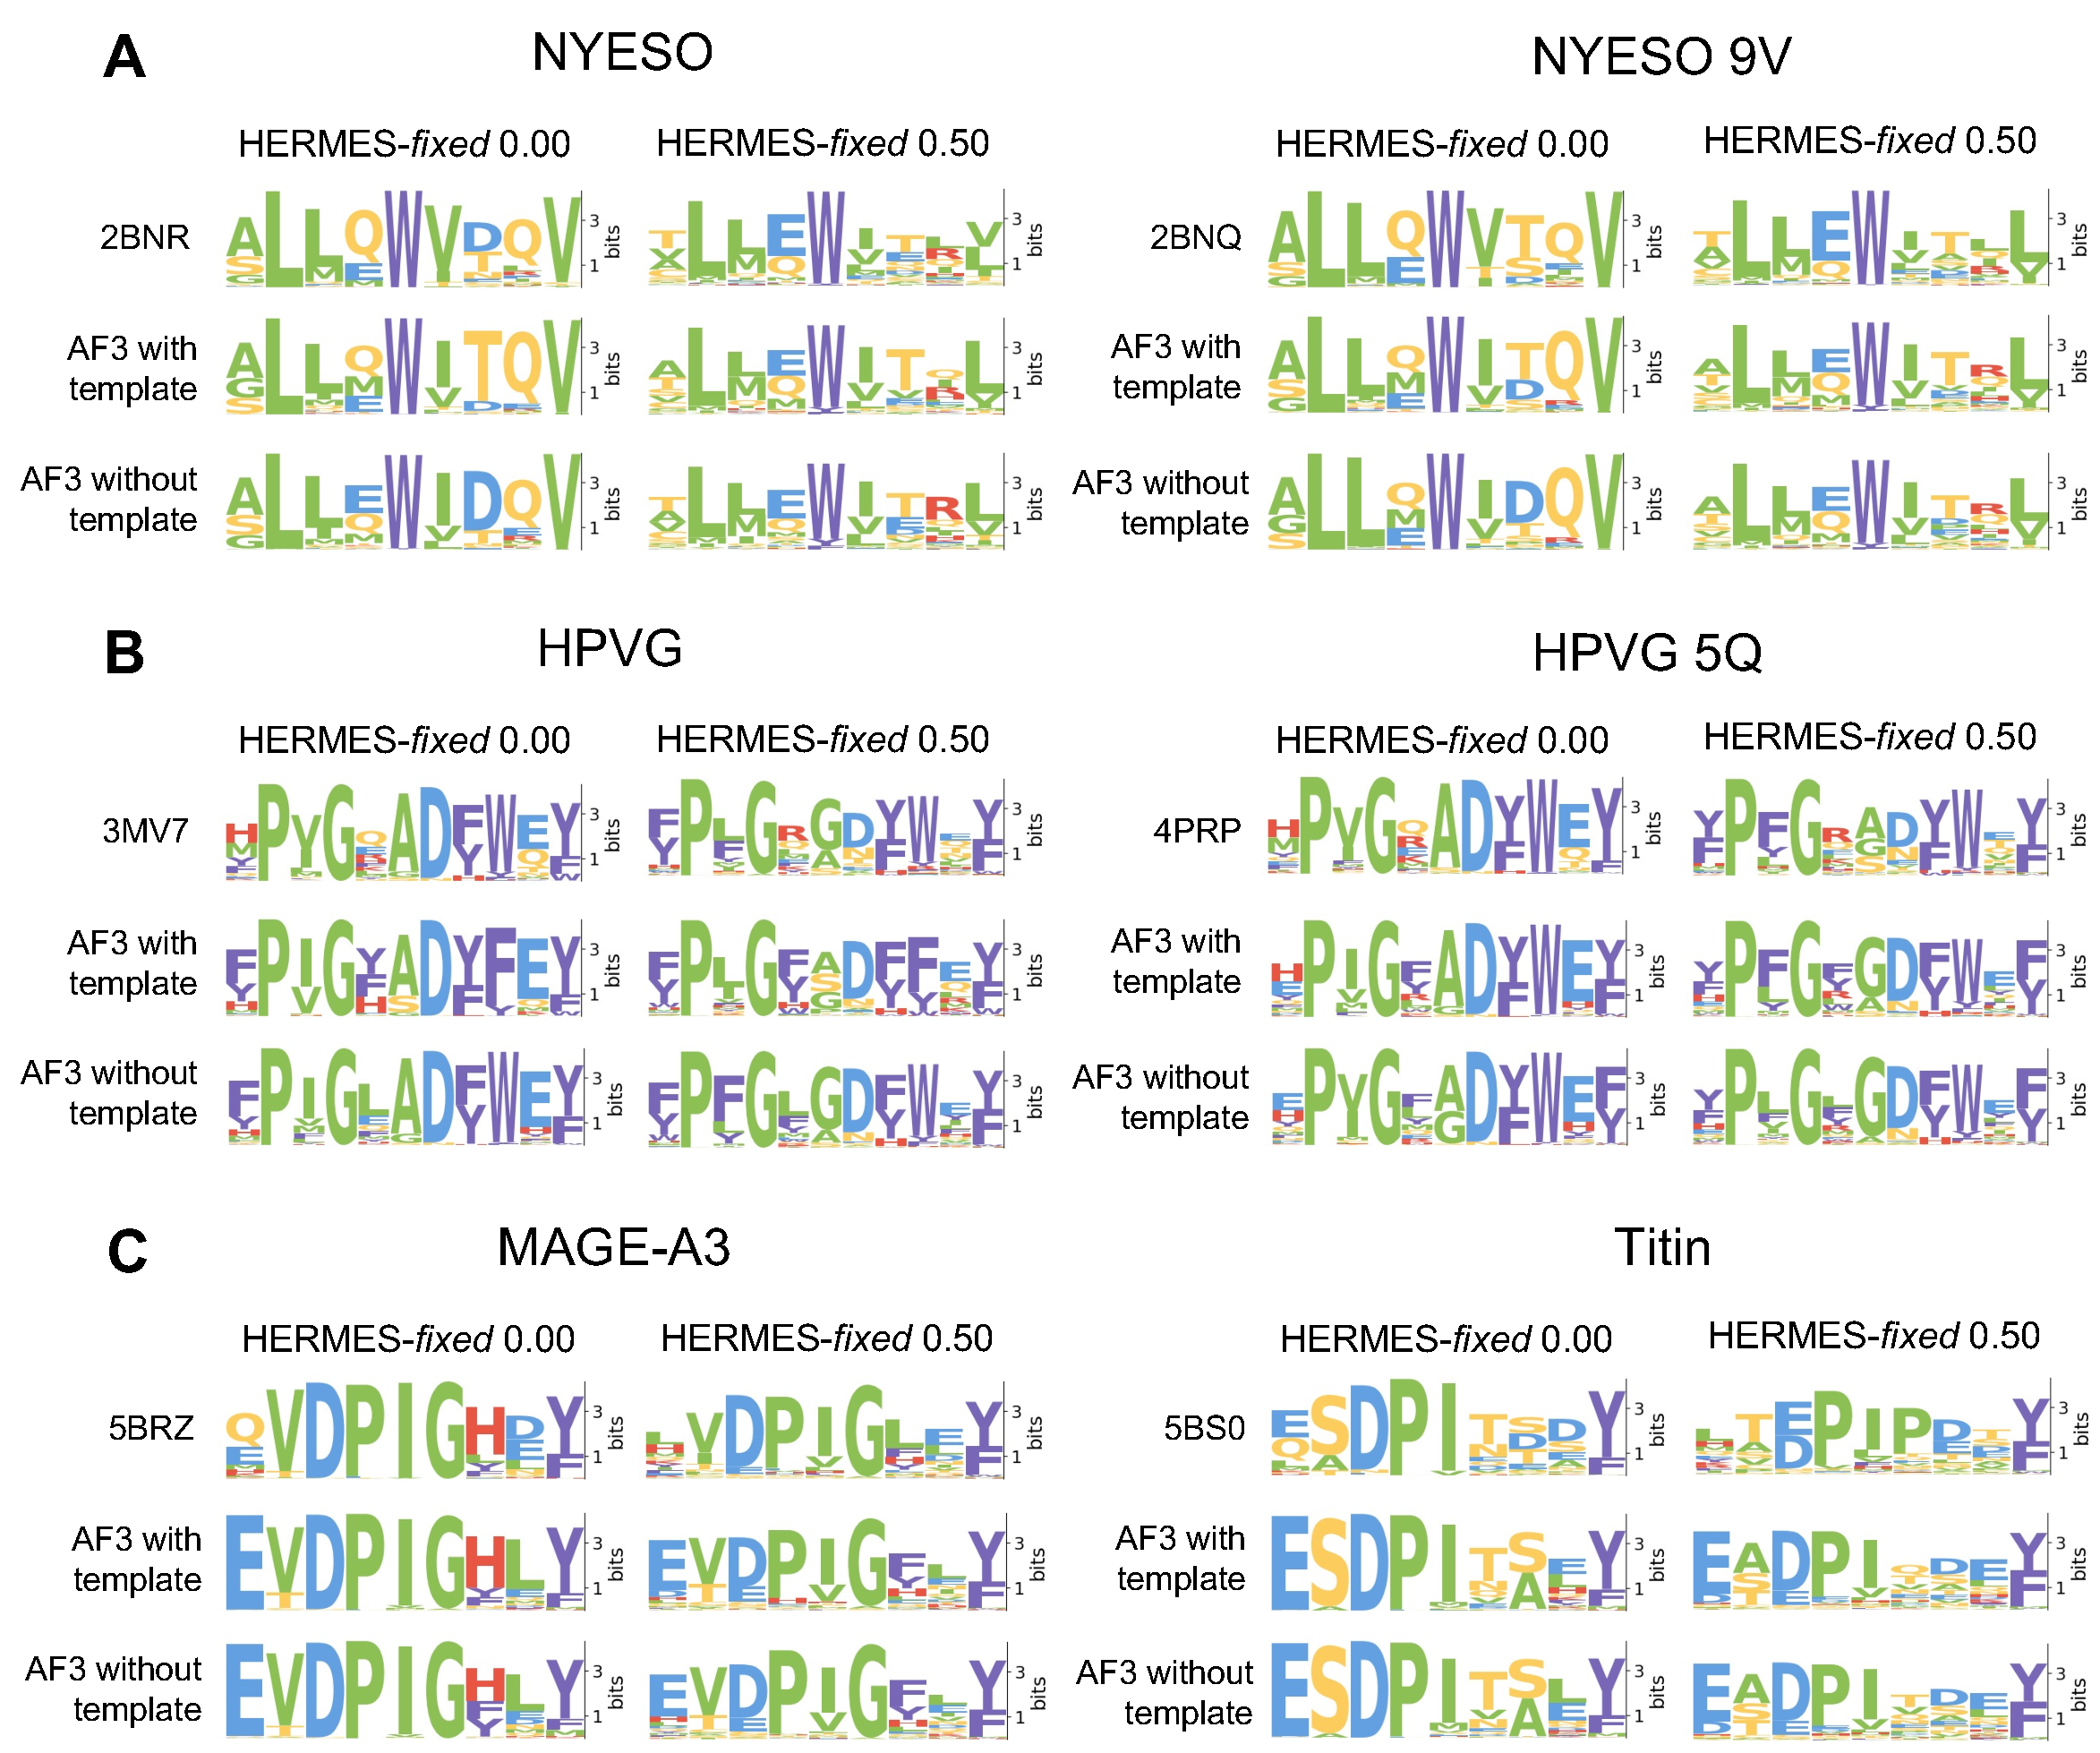
\includegraphics[width=1.0\textwidth]{figures/joint_logoplots_for_design.pdf}
\figcaption{Composition of designed peptides using experimental versus AlphaFold3 structures as
design templates.}{ For the {\bf(A)} NY-ESO, {\bf(B)} EBV, and {\bf (C)} MAGE, each panel displays
the position weight matrices (PWMs) for peptides designed using the HERMES-{\em fixed} protocol.
Designs were generated using three types of structural templates as indicated in each panel: the
experimentally determined wild-type structure (first row), and the AlphaFold3-predicted models of
that structure generated with (middle) and without (bottom) template guidance. PWMs are shown
separately for the HERMES-{\em fixed} models trained with different noise amplitudes (as indicated
above the panels). For each system, results are provided for the two wild-type peptides used as
input structural templates (shown in the left and right columns of each panel).
}
\label{fig:joint_logoplots_for_design}
\end{figure}






\begin{figure}[ht]
\centering
	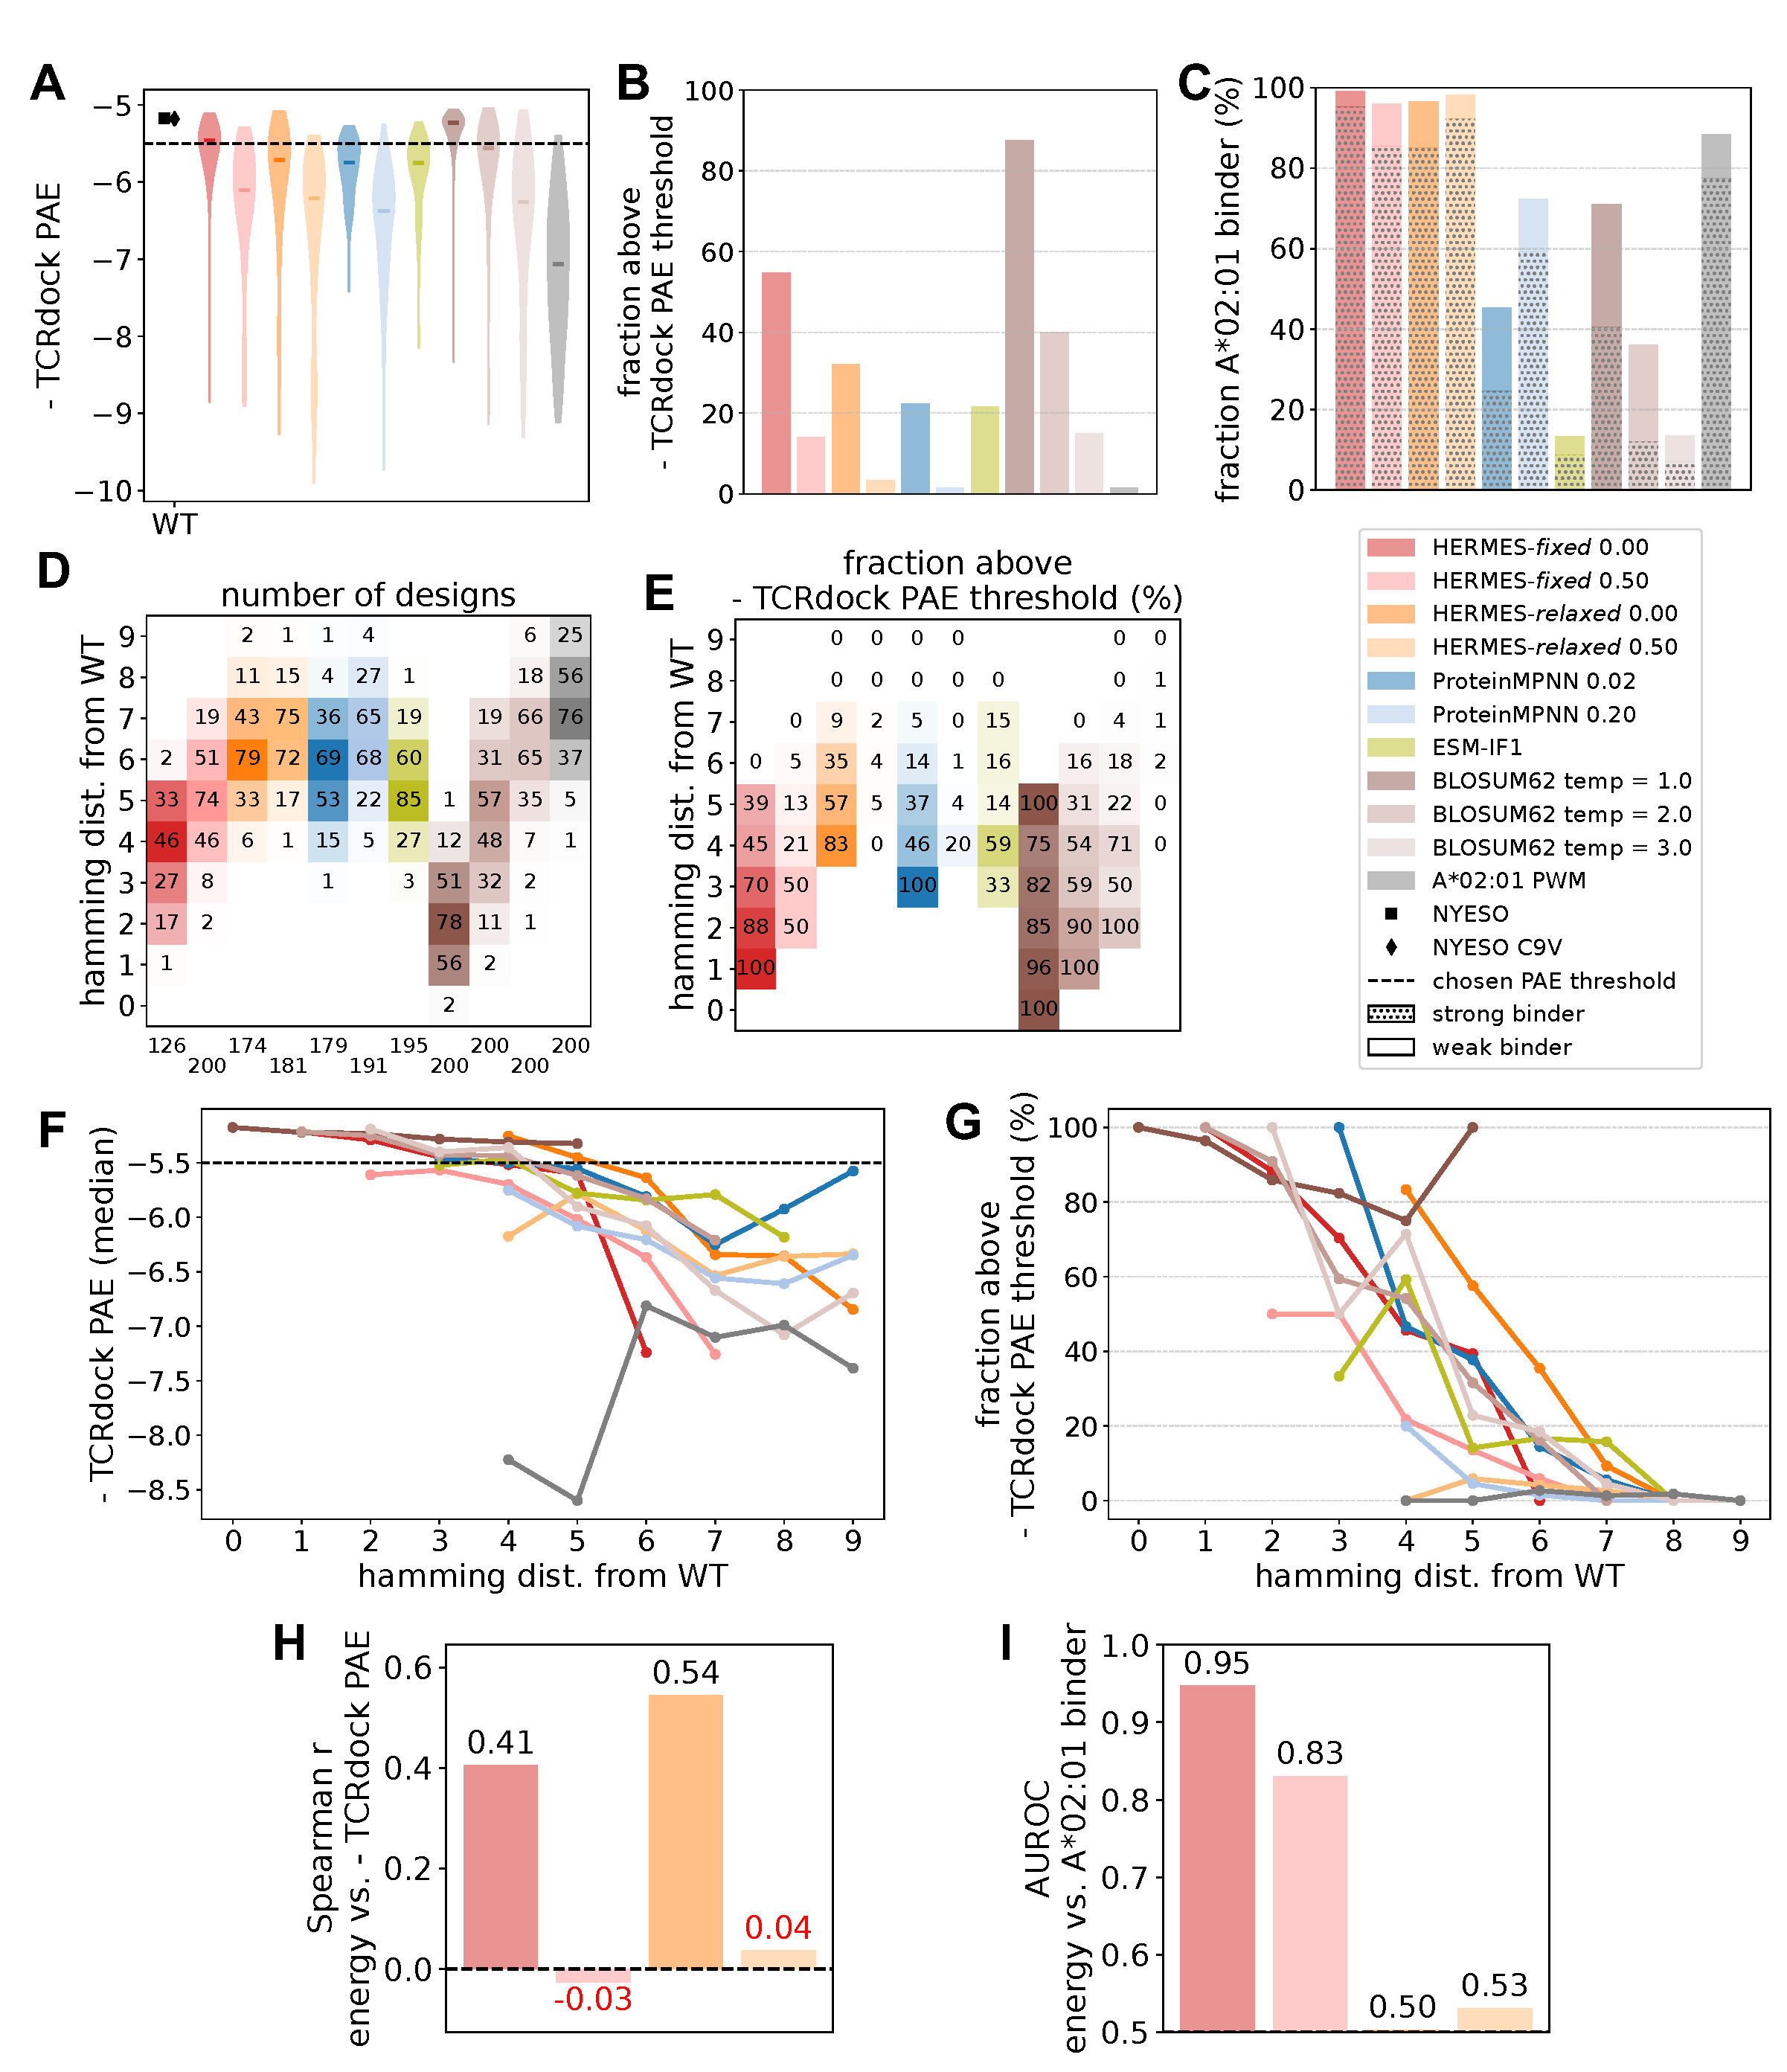
\includegraphics[width=0.9\textwidth]{figures/design_tcrdock_nyeso.pdf}
\figcaption{Benchmarking of models for peptide design in the NY-ESO system.}{
\textbf{(A)} The distribution of the TCRdock negative-PAE's for peptides designed by different
computational protocols (colors) are shown; in each case the score distribution for 100
independently designed peptides is shown. The horizontal dashed line indicates the PAE threshold
chosen to classify positive designs.
\textbf{(B)} The fractions of designed peptides that pass the TCRdock PAE threshold is shown for
each method.
\textbf{(C)} The fraction of designs that are predicted by
NetMHCPan~\cite{reynisson_netmhcpan-41_2020} to be presented by the template's MHC allele are shown;
dotted regions correspond to strong binders (EL\_rank $\leq 0.5$), while the bar indicates all weak
and strong binders (EL\_Rank $\leq 2.0$). HERMES designs are most consistently predicted to be
presented by the MHC.
\textbf{(D)} The number of designs, and {\bf (E)} the fraction of designs that pass the TCRdock PAE
threshold are shown for each model (colors) at different Hamming distances from the wild-types; The
numbers at the bottom of each column in (D) indicate the total number of unique designs.
{\bf (F)} The median of TCRdock negative-PAE across designs, and {\bf (G)} the fraction of designs
that pass the TCRdock PAE are shown for each model (colors) as a function of the Hamming distance
from the wild-types.
{\bf (H)} Spearman correlation between HERMES-predicted peptide energy and TCRdock PAE is shown,
with data pooled across design models. In each case, HERMES energies are computed using the same
protocol applied during design. Correlations that are not statistically significant (p-value $>
0.05$) are highlighted in red.
{\bf (I)} Shows the AUROC for classifying whether a designed peptide is presented by the template's
MHC allele (i.e., predicted to be a strong binder according to
NetMHCPan~\cite{reynisson_netmhcpan-41_2020}), using HERMES peptide energy as the classifier. As in
(H), for each peptide, HERMES energies are computed via the same protocol used for their deign.
The HERMES model names specify the design scheme (fixed, relaxed), and the noise amplitude (in \AA)
injected to the coordinates of the structure data during training. The ProteinMPNN design uses
baseline scoring scheme with peptide 1-by-1 (eq.~\ref{eq:peplogp_proteinmpnn}), with the training
noise amplitude specified in the model name.}
\label{fig:design_tcrdock_nyeso}
\end{figure}



\begin{figure}[ht]
\centering
	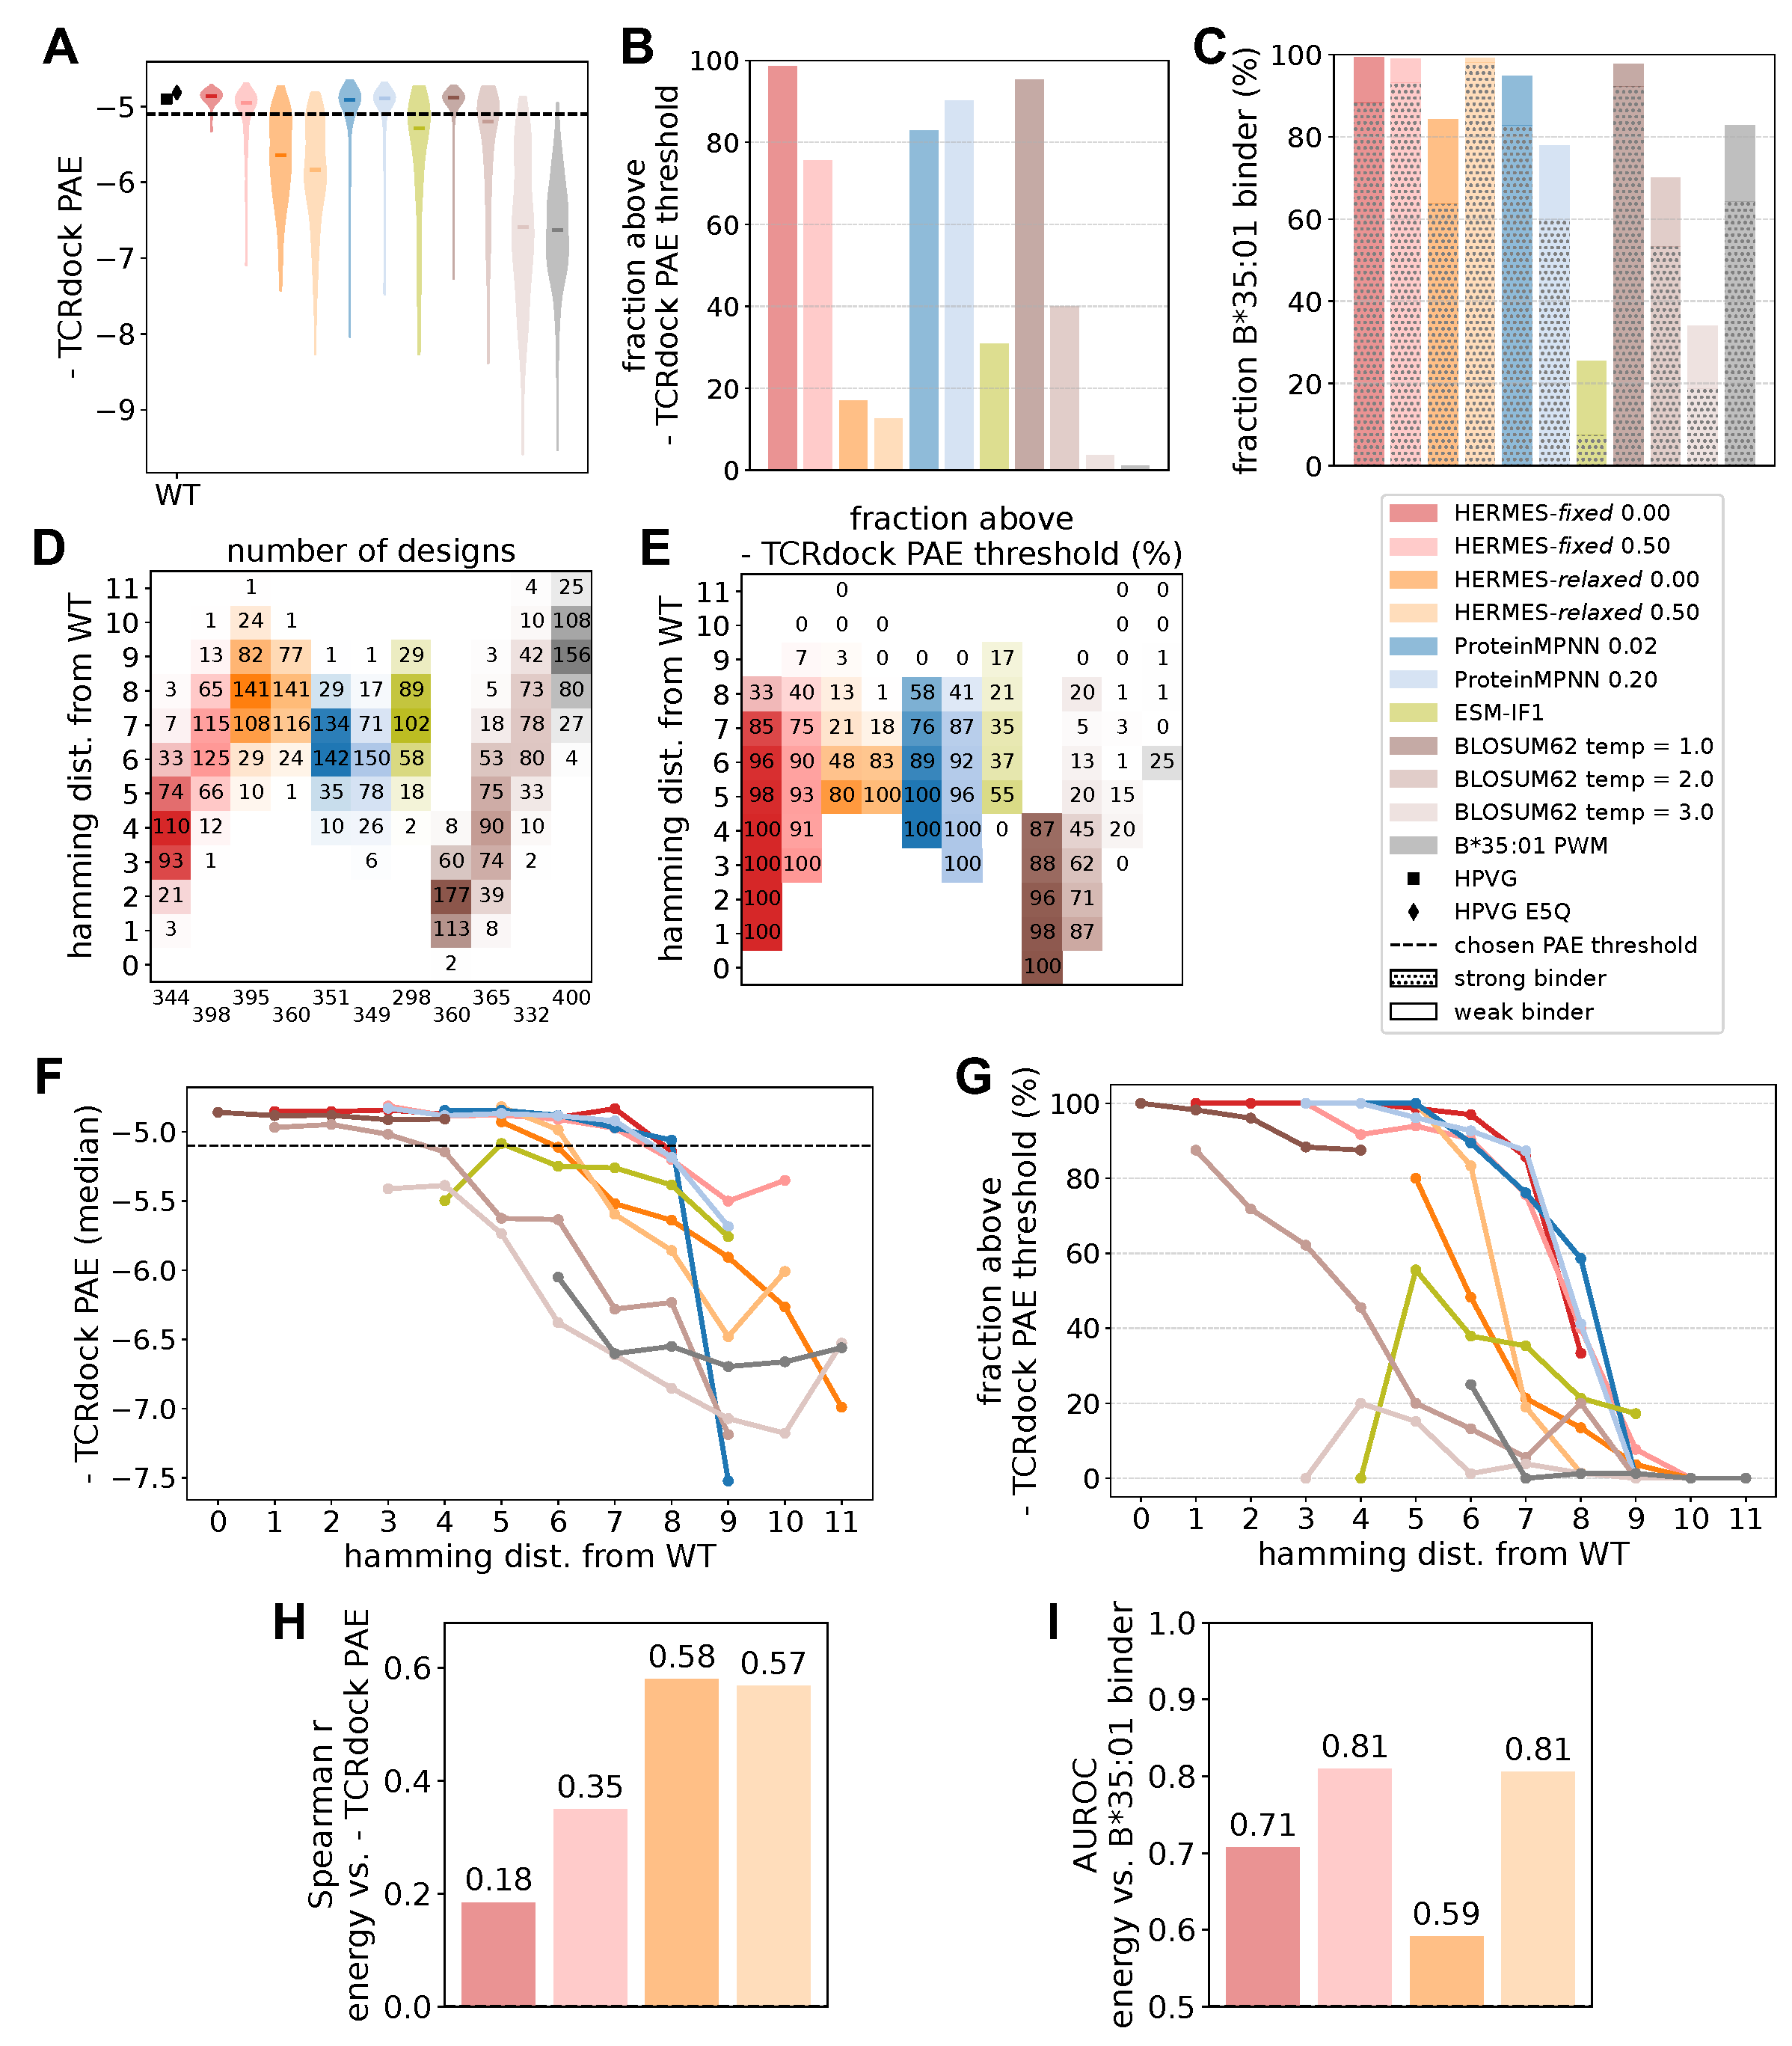
\includegraphics[width=0.9\textwidth]{figures/design_tcrdock_ebv.pdf}
\figcaption{Benchmarking of models for peptide design in the EBV system.}{ Similar to
Fig.~\ref{fig:design_tcrdock_nyeso} but for the EBV system.}
\label{fig:design_tcrdock_ebv}
\end{figure}



\begin{figure}[ht]
\centering
	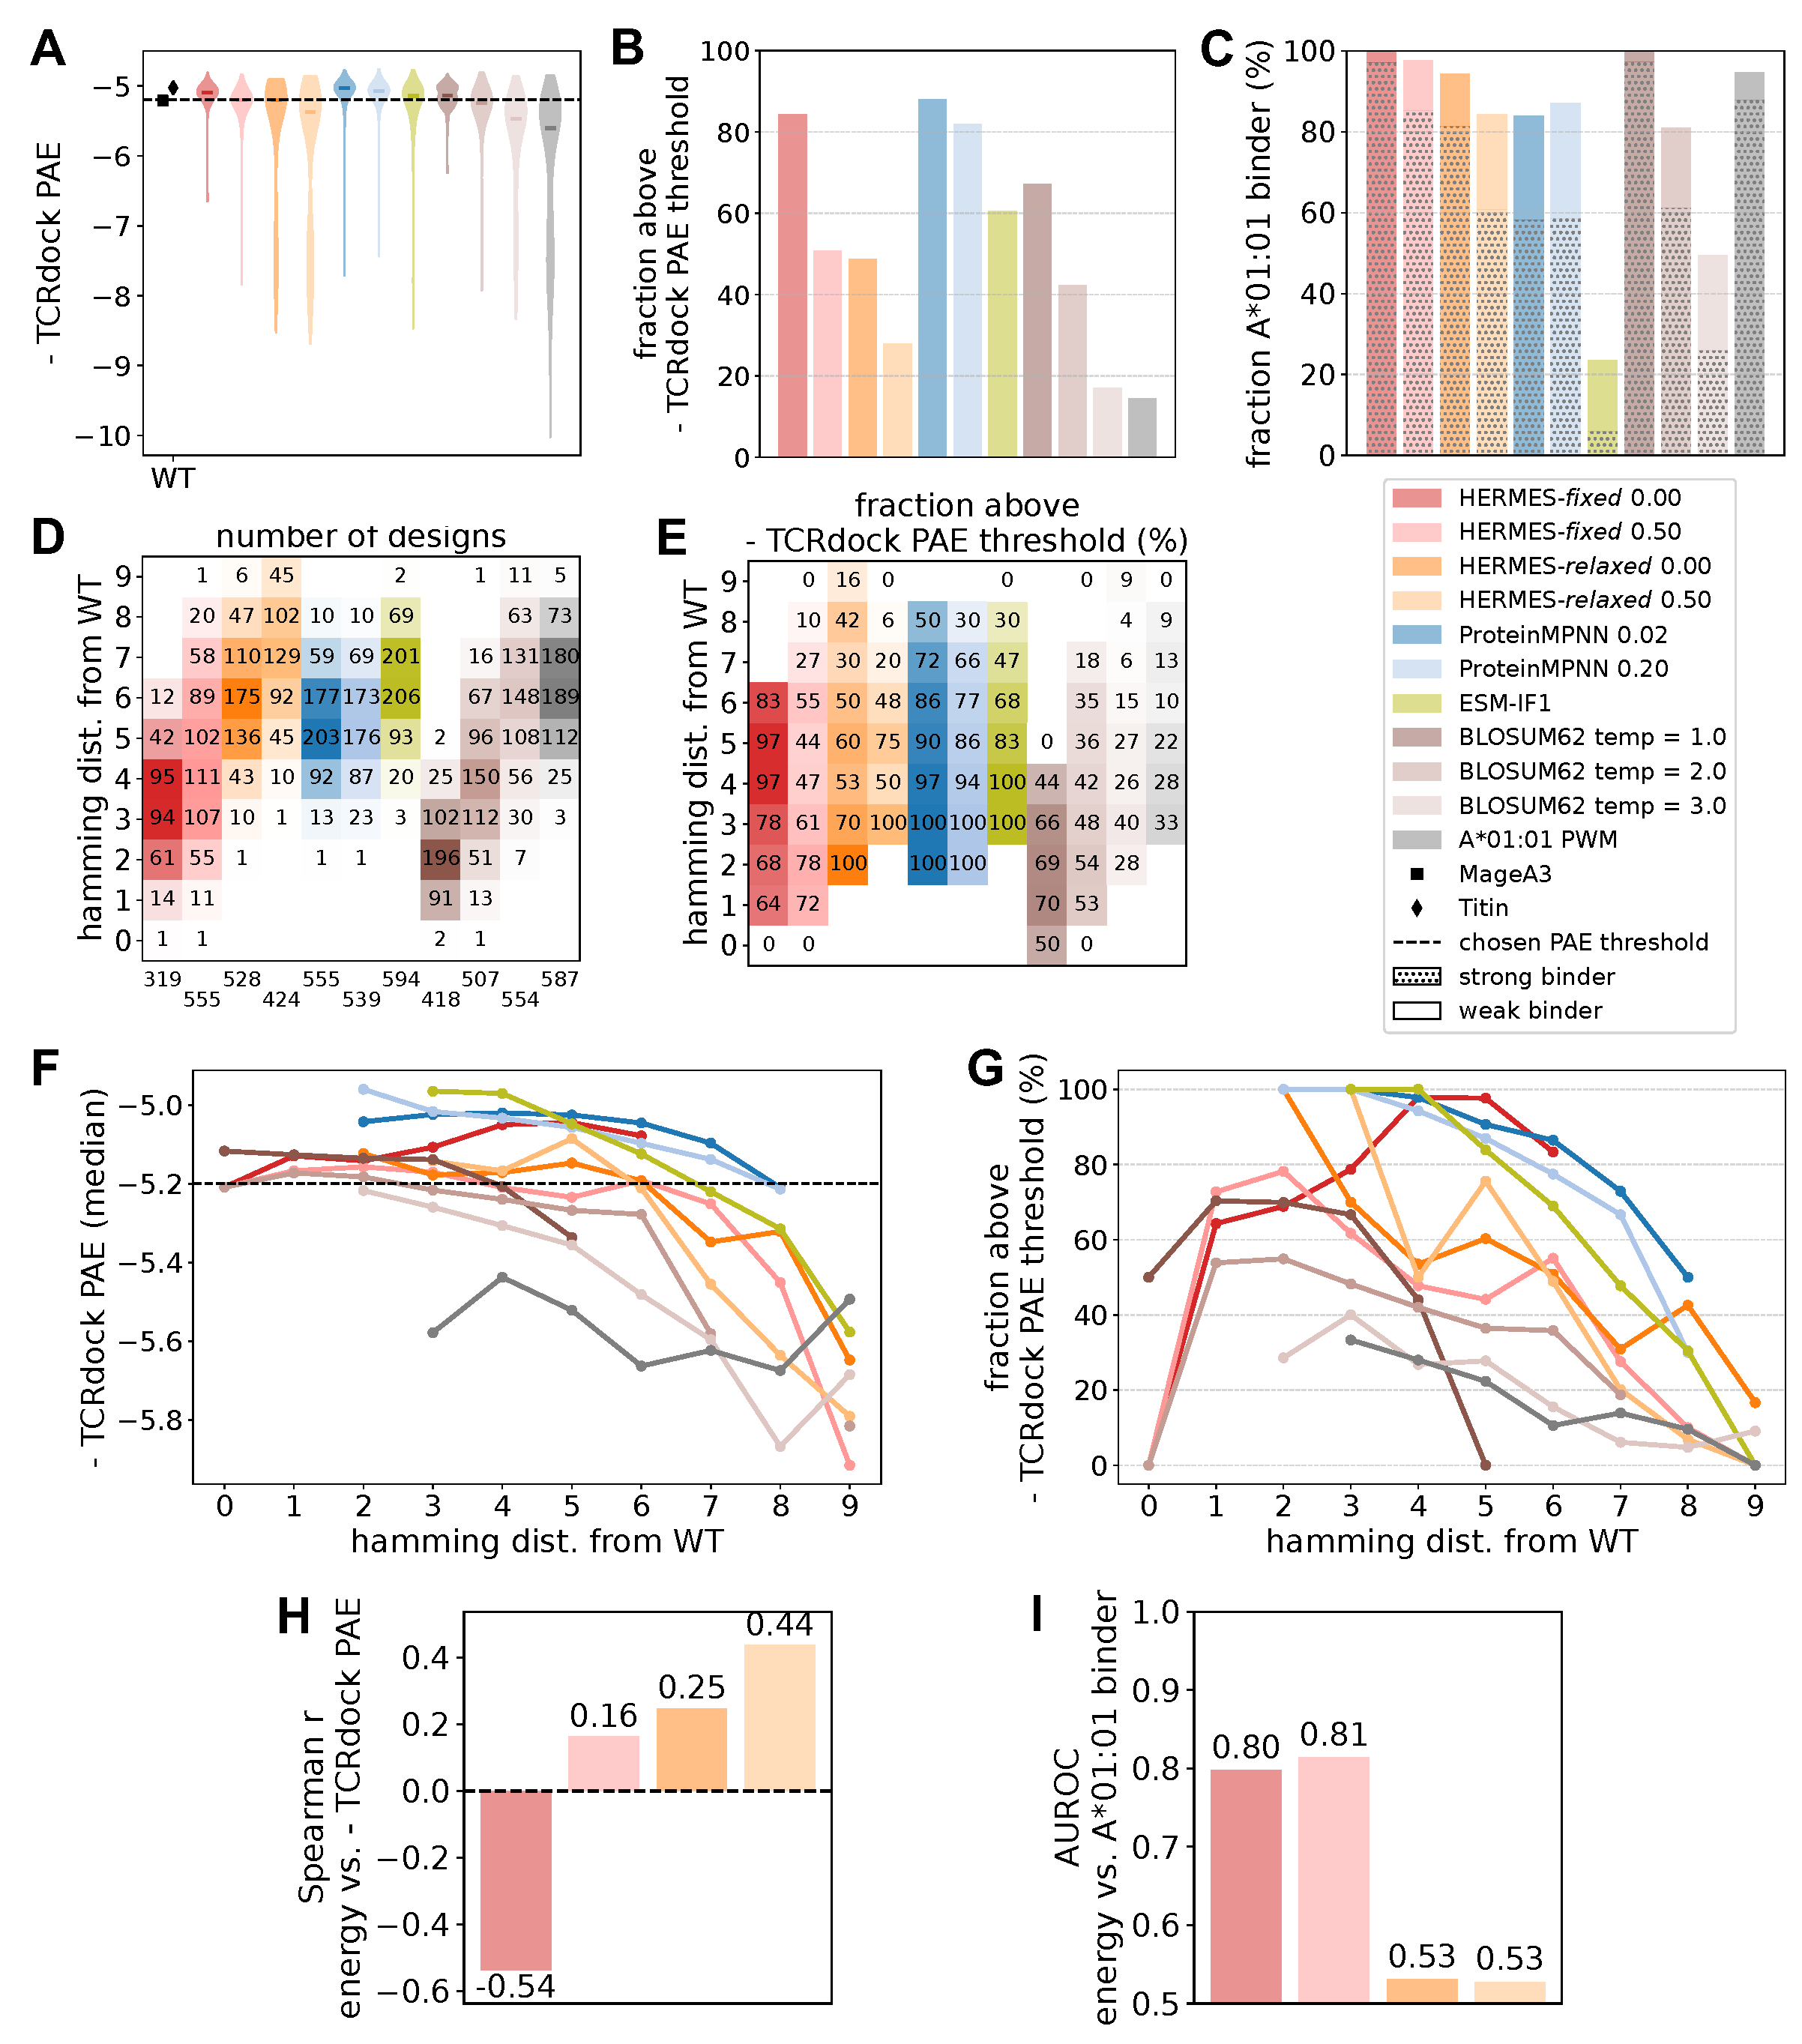
\includegraphics[width=0.9\textwidth]{figures/design_tcrdock_mage.pdf}
\figcaption{Benchmarking of models for peptide design in the MAGE system.}{ Similar to
Fig.~\ref{fig:design_tcrdock_nyeso} but for the MAGE system.
}
\label{fig:design_tcrdock_mage}
\end{figure}

\begin{figure}[ht]
\centering
	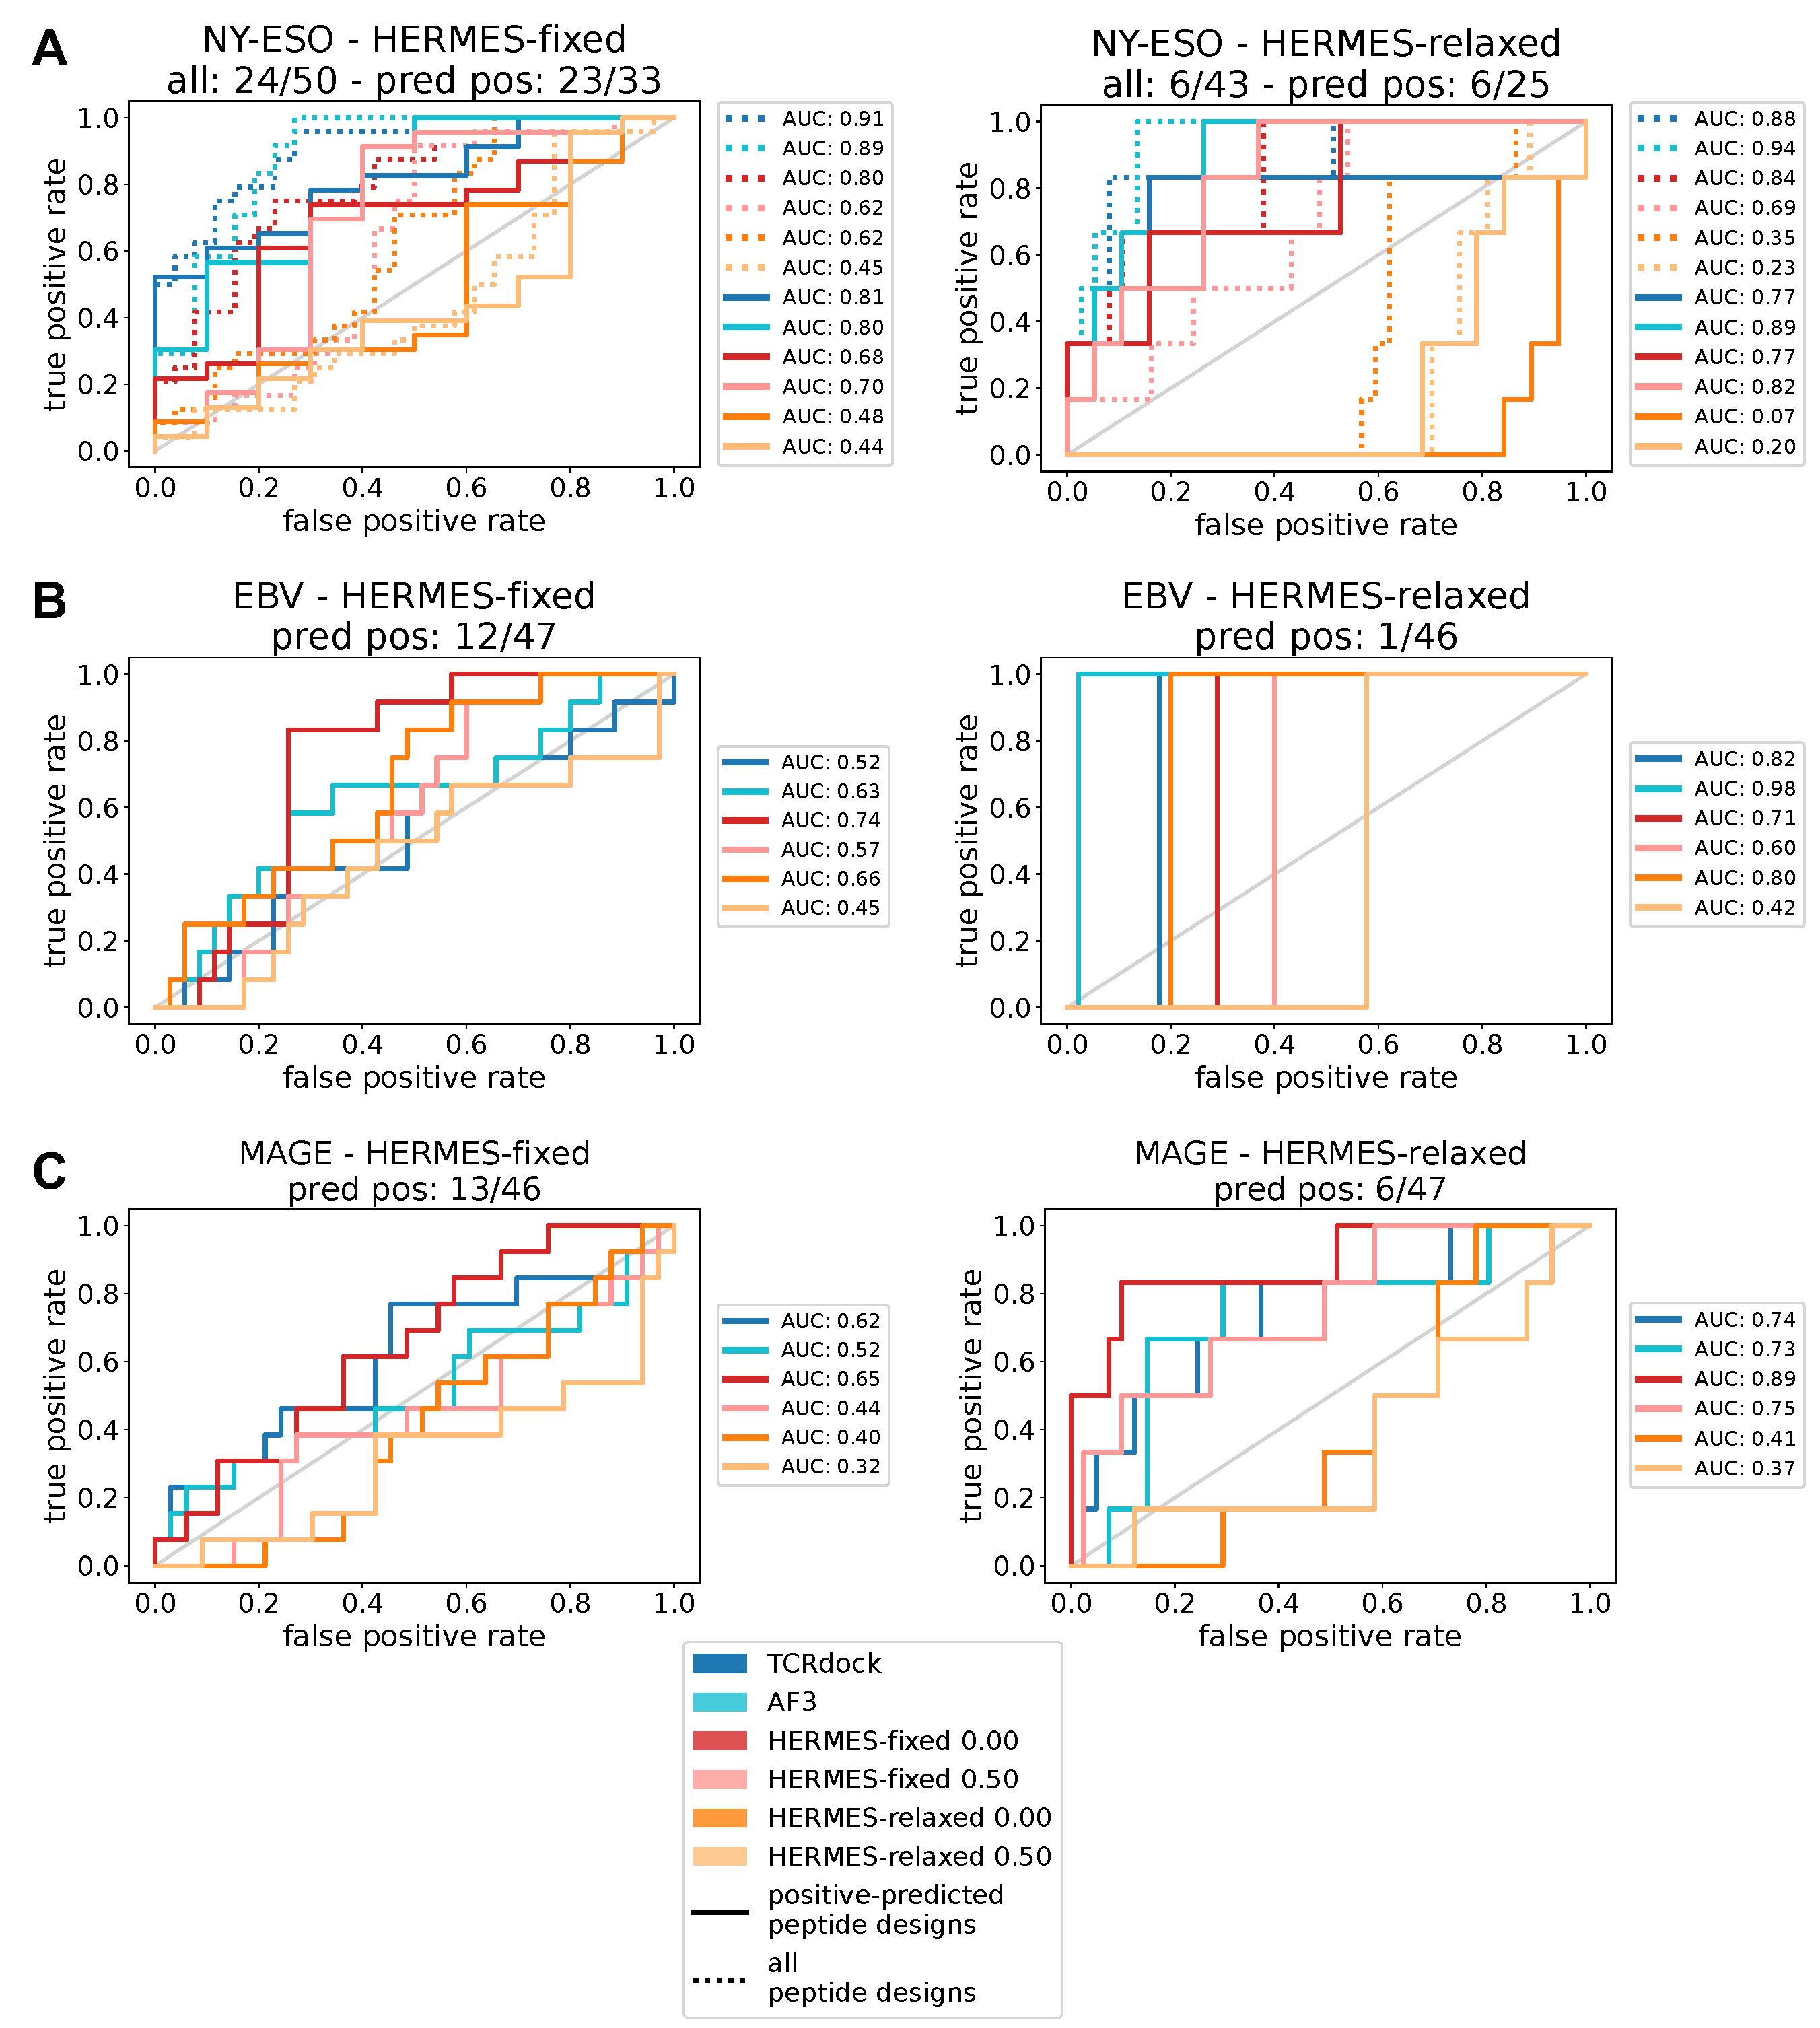
\includegraphics[width=0.8\textwidth]{figures/roc_curves.pdf}
\figcaption{Discrimination ability of different scoring schemes as design filters.}{
The ROC curves show true positive versus false positive rates when using scores from different
models--HERMES, AlphaFold3, and TCRdock (color coded as in the legend)--as scoring criteria for
peptide design. Results are shown separately for designs generated using the HERMES-{\em fixed}
(left) and the HERMES-{\em relaxed} (right) protocols, for the {\bf (A)} NY-ESO, {\bf (B)} EBV, and
{\bf (C)} MAGE systems. Experimentally measured peptide-induced T-cell activity (GFP\%) is used as
the ground truth for evaluating the predictive performance in each case. {For the NY-ESO system only
{(A)} we show ROC curves computed on both peptides that were predicted to activate T-cells
(positives) based on their TCRdock PAE scores (full lines), and the mixture of positive and negative
peptides (dotted lines). For EBV and MAGE {(B-C)}, the scoring criterion is only tested for the
peptides that we deemed to be activating (positive) based on their TCRdock PAE scores (full lines),
as these were the ones that we tested experimentally. } The HERMES model names specify the design
scheme (fixed, relaxed), and the noise amplitude (in \AA) injected to the coordinates of the
structure data during training.
}
\label{fig:design_roc_curves}
\end{figure}



\begin{figure}[ht]
\centering
	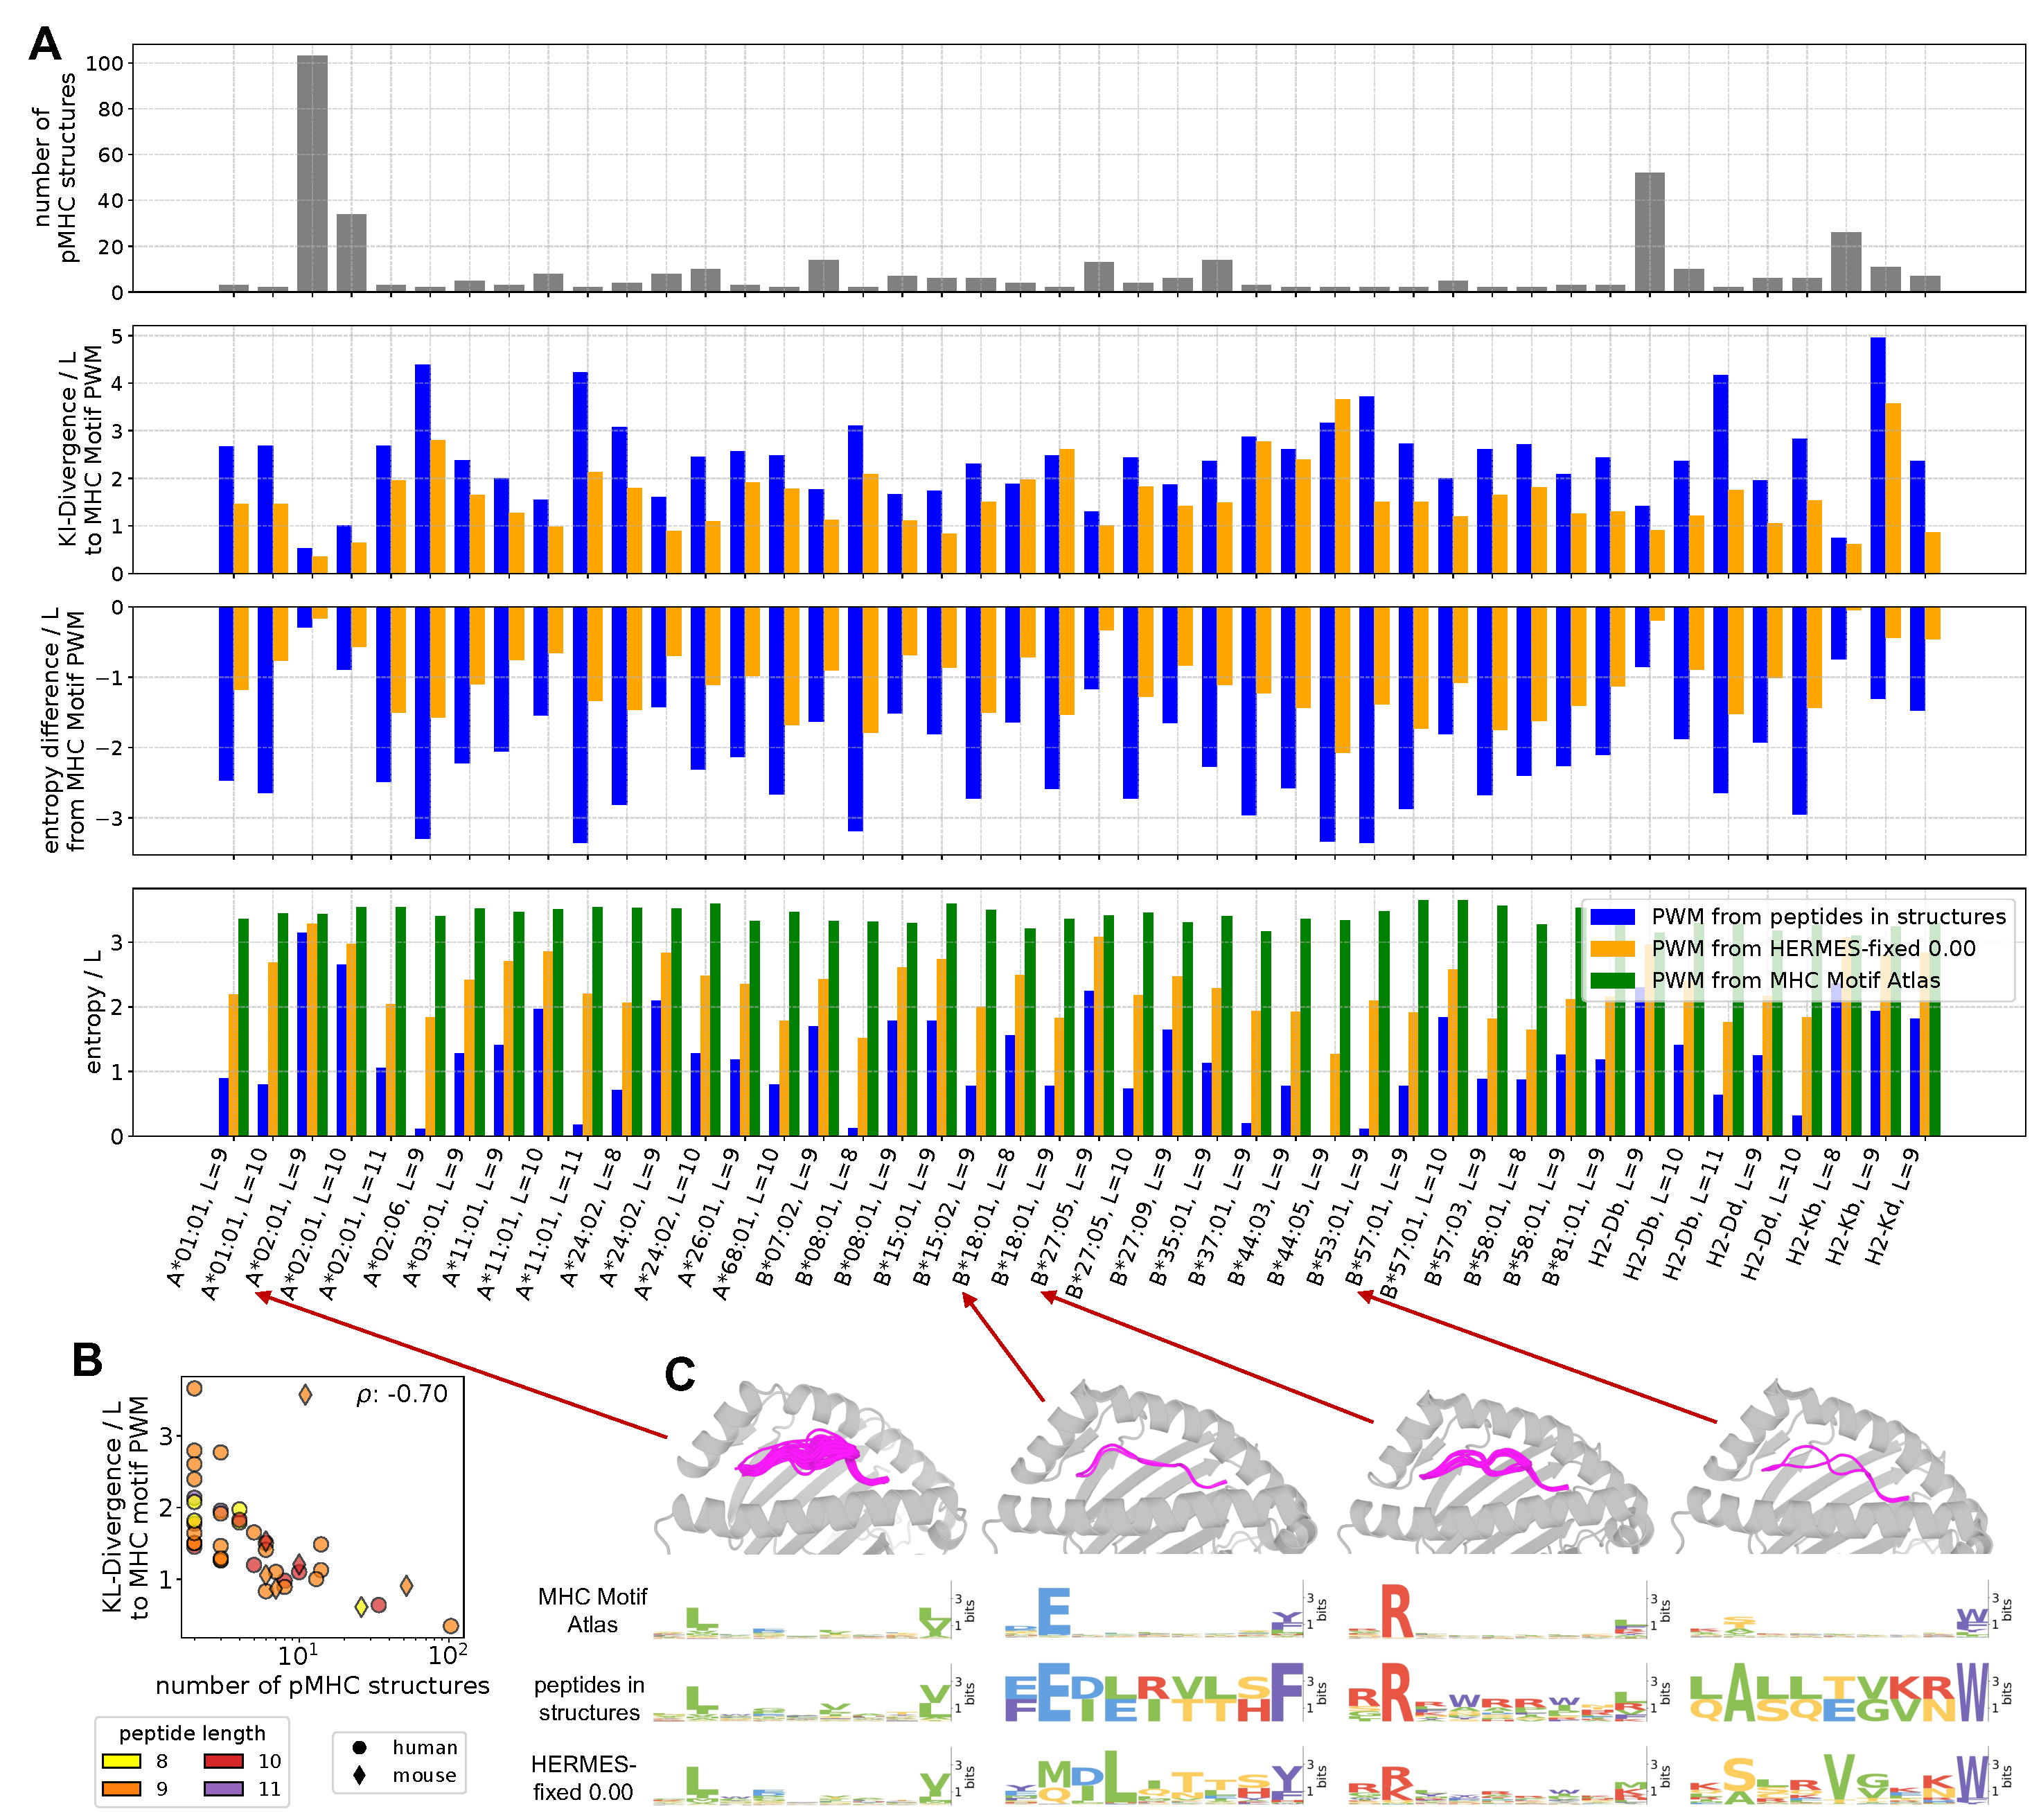
\includegraphics[width=1.0\textwidth]{figures/pmhc_pwm_entropy_comparisons.pdf}
\figcaption{Predicting MHC-I peptide presentation preferences with HERMES.}{
We evaluated HERMES's ability to recover MHC class I peptide presentation preferences by analyzing
pMHC structures from the TCR3d database~\cite{gowthaman_tcr3d_2019}, grouped by MHC allele and
peptide length (L), retaining only those combinations with at least two structures. As ground truth,
we used position weight matrices (PWMs) from the MHC Motif Atlas~\cite{Tadros2023-ij}, derived from
large datasets of peptide sequences known to be presented by each allele.
HERMES-{\em fixed} was used to design peptides for each structure in a given allele-length group,
and the resulting PWMs were averaged across structures to generate a motif reflecting the peptide
preferences for that MHC I allele (for a given length).
As the baseline, we used PWMs generated directly from the peptides found in the structural dataset.
PWM quality was evaluated using the Kullback-Leibler divergence, and the entropy difference from the
ground-truth PWM. {\bf (A)} Shown are the summaries of data and performances across all MHC I
allele-length combinations: number of available structures (first row), KL-divergence between the
HERMES-derived PWMs (or the baseline) to the ground truth (second row), the entropy difference to
the ground truth (third row), and the entropy of the PWMs based on the three approaches (fourth
row). {\bf (B)} Shown is the KL-divergence of HERMES-derived PWMs versus the number of available
pMHC structures for across different allele-length classes. {\bf (C)} Examples of pMHC structures
and the corresponding PWMs are shown for four allele-length combinations, spanning a range of
structure counts. In each case, structures are aligned along the MHC chain to show the diversity of
peptide poses captured by the ensemble of available structures, used as design templates. }
\label{fig:pmhc_pwm_entropy_comparisons}
\end{figure}


